                                                                                                                                                                                                                                                                                                                                                                                                                                                                                                                                                                                                                                                                                                                                                                                                                                                                                                                                                                                                                                                                                                                                                                                                                                                                                                                                                                                                                                                                                                                                                                                                                                                                                                                                                                                                                                                                                                                                                                                                                                                                                                                                                                                                                                                                                                                                                                                                                                                                                                                                                                                                                                                                                                                                                                                                                                                                                                                                                                                                                                                                                                                                                                                                                                                                                                                                                                                                                                                                                                                                                                                                                                                                                                                                                                                                                                                                                                                                                                                                                                                                                                                                                                                                                                                                                                                                                                                                                                                                                                                                                                                                                                                                                                                                                                                                                                                                        \documentclass[english]{tktltiki}
\usepackage[pdftex]{graphicx}
\usepackage{subfigure}
\usepackage{url}
\usepackage{amsmath}
\usepackage{tikz}
\usepackage{multirow}

\begin{document}
%\doublespacing
%\singlespacing
\onehalfspacing

\title{A formal study on Content Based Image Retrieval systems}
\author{Sayantan Hore}
\date{\today}

\maketitle

\numberofpagesinformation{\numberofpages\ pages + \numberofappendixpages\ appendices}
\classification{\protect{\ \\
A.1 [Introductory and Survey],\\
I.7.m [Document and text processing]}}

\keywords{layout, summary, list of references}

\begin{abstract}

Content based image retrieval systems are out there for a few years now. We present a system, IMSE, here which searches out images using Gaussian Process Upper Confidence Bound algorithm. This algorithm has performed better in comparison to random search and plain exploration. We present a comparison of how the algorithm performs on CPU as well as GPU. We also evaluate the user experience and with the search interface.

\end{abstract}

\mytableofcontents




\section{Introduction}

With the advent of digital media, searching for media contents, especially images, became essential. Until recent, there has been no convenient technique to search for images. Traditional computing machines, equipped with text-input devices, like keyboard, allow users to enter texts only as a search query. This has been useful for text based information retrival because, as the search query and the content being searched for are texts, having letters as common building blocks, the input can directly be mapped to the search space. This can be referred to as direct searching.

Images are not built with letters, so in case of a text based search, the keywords in the search query have to be mapped to the images first. Therefore this is indirect searching. To achive this mapping, all the available images have to be annotated or tagged. This annotation involves manual labour. Moreover, annotation can be wrong, also some images might not receive annotation at all. These lead to inappropriate search results. We will highlight three different cases below.

Say, somebody has a pet dog named "Tiger". A photograph of the dog, tagged as "Tiger" is uploaded to a social media image database. Now if somebody is searching for a tiger in its true sense, it is very common that the system can include the photograph of that dog into the search result. As the system is not searching by the contents of the images, it cannot differentiate between two pictures with a same tag.

Say, the owner of "Tiger" forgot to attach a tag to the picture. Somebody, searching for dogs, would not receive the photograph of "Tiger". This is unacceptable.

Say, somebody is searching for blue whales. The system will try to find different combinations of search keywords. Therefore it is common to get multiple images, some of them being whales, and the rest anything blue, like a blue shirt. The system cannot go inside a picture to see whether the whale present there is blue or not. A blue whale can only be retrieved if either the whale in the picture is actually a blue one, or it is tagged as "blue whale".

To tackle these issues, it is required to search for and by the actual contents of images. Contents of images can be represented on a computer as features like RGB colour space, colour gradient, texture, shape etc. These representations are all numeric values. If all the images present are numerically represented in features, they can be searched for by feature values. This image retrieval procedure is known as \textit{content based image retrieval} or CBIR. A lot of researchers have been trying to build such systems over the past few years. There are some good systems there that involves various image features and apply machine learning techniques to retrieve images. Some of them use a supervised learning approach to train a learning agent, but it is time consuming to train an agent before it can go live and perform. We have built a small and simple system which include only colour as a feature but instead of using supervised learning, we use reinforcement learning technique. Here the learning agent interacts with the user and from the user interactions it learns what the user likes and recommends images accordingly. There is no need to train it offline. We use \textit{Gaussian process bandits} in reinforcement learning setting to retrieve relevant images. In the subsequent sections we include the necessary theoretical background, a brief description of similar but relevant systems, construction of our system following the theory given, experiment setup and conclusion. 

\iffalse
Content based image retrieval systems have been proven to fit better in retrieval performance. Text or tag based matching systems rely only on texts, thus the images themselves are secondary in the search procedure. The user sees the image and selects one by the objects and color the image represents. The combination of those objects and colors should actually be searched for instead of tags. Tags hardly represent an entire image. An image portraying a cloudy afternoon can be tagged as "Sad", based on the mood and understanding of the person creating the tags. Another image of the same genre, tagged by different persons, might miss the tag. If a user is in search for "Sad" images and finds one with the tag, selects it. The other "Sad" image would not appear in the search results as it lacks the tag. Had features and content of the image been searched for, we could get better and more appropriate search results.

IMSE is a content based image retrieval system, using Gaussian Process Upper Confidence Bound (GP-UCB) as a retrieval algorithm. We are using MIRFLICKR 25000 \cite{mirflickr} image set for testing. As this produces a huge kernel, GP-UCB is slow on CPU. We have written a GPU version of the algorithm and made a comparative study of running time over CPU and GPU. The system is written in Python (and Django for the web interface). Any system has to have a pleasing and assisting user interface. As our system is targeted towards web users, we cared for having a decent web interface, written in Twitter Bootstrap (v3.0) framework, jQuery (v1.11.1), CSS and javascript. We have followed Human Computer Interaction guidelines for user interaction.

In subsequent section, we will present the theoretical background of Reinforcement Learning, Gaussian Process, Upper Confidence Bound, Image Retrieval, GPU implementation details, user experience and performance measures.


\section{The need for content based retrieval in detail}

...

\subsection{Shortcomings of traditional image search}
%\enlargethispage{5mm}

...

\subsection{Why content based retrieval is better}


...


\subsection{Approaches}

...

\fi

%\pagebreak

\section{Theoretical background}

Here we discuss the theoretical background necessary for understanding the modelling of image retrieval, especially the model we went for. We discuss reinforcement learning, bandit problems, upper confidence bound, regression problems, Bayesian probability model, Gaussian process and application of Gaussian process in bandit problems one by one.


\subsection{Reinforcement Learning}

Reinforcent learning \cite{reinforcement_learning} is a form of machine learning in which the learning agent interacts with its surroundings, by performing an action. The surroundings or the environment reacts by giving some feedback to the agent. The feedback, perceived to be either positive or negative, helps the agent to understand whether the action was correct or incorrect respectively. The feedback is considered as a reward associated with the action performed. The agent has a goal to reach which is quantified as receiving the maximum cumulative reward after a finite sequence of actions. A system modelled after reinforcement learning, has a finite number of states $S = \{s_1, s_2, ..., s_n\}$. The agen starts from a state $s_i$ and tries to reach a \textit{goal state} $s_j; j \neq i$. Any state $s_k \in S$ has a set of actions $A = \{a_1, a_2, ..., a_m\}$ associated with it. The agent while being in $s_k$ can perform any one of the available actions. It receives a reward $r_k$, which is positive if the action takes the agent closer to the goal state $s_j$, otherwise negative. Clearly the same action (moving forward or backward for example), associated to more than one different states, can produce different rewards depending on starting state, goal state and the position of current state in between. The task of learning here is to predict the reward for a particular action given the state. As the agent goes through trials, it gathers knowledge or inference about the outcome of an action for a state in terms of rewards, as it receives an immediate reward for each action performed. The knowledge of the agent, about different combination of state-action pairs, is reinforced real time.

Reinforcement learning is fundamentally different from two other major form of learnings, supervised and unsupervised learning. Neither it tries to classify a new unlabeled dataset based on already labeled dataset, nor it  finds patterns in a new dataset. It rather tries to understand an environment which can react on its action. It is therefore useful in applications of game theory, robotics, web advertisement, product recommendation in online stores etc. In all these cases there is an active party providing rewards on an action. For example in product recommendation in an online store, the system, acting as an agent, recommends a product and the customer, acting as the environment, can either choose the product or not, thus generating positive or negative reward resprectively.

\subsubsection{Exploration and Exploitation}

There are problems where there is an infinitely large state-action pairs but the agent has to reach the goal state in finite steps. Clearly, the shortest path generates the maximum reward. As the step size is finite, the agent cannot try each available state-action pair. In each state it visits, it would rather try to repeat the action that has generated the maximum reward so far. This way it might miss an action in a particular state that could generate a bigger reward. Again one action might generate a lower immediate reward in a state but it might be a keypoint that follows a shorter path than the known one to the goal state thereafter, thus contributing to a bigger overall gain. The agent has two problems here, firstly, as it has to achieve the goal in finite time, it cannot go through all possible combinations (i.e. \textit{exploration}) much. Secondly, always performing the best known action (i.e. \textit{exploitation}) might miss a better action. This situation is known as exploration-exploitation \cite{reinforcement_learning} dilemma. There exist some solutions to this problem depending on the nature of the problem. In a simple reinforcement learning problem we apply \textit{epsilon-greedy} or $\epsilon$ \textit{-greedy} \cite{reinforcement_learning} method to control the amount of exploration by a probabilistic measure $\epsilon$. In bandit problems, the amount of exploration is controlled by upper confidence bound, a quantity probabilistically calculated. We will discuss all these later.

\subsection{Bandit Problems}

Bandit problems \cite{bandits} are sequential decision problems where each iteration in the sequence has multiple choices of actions. Each action is associated with a distribution of numerical rewards. Each action also leads to an observation which is a reward value from the associated distribution. The goal is to maximise the reward over a finite number of trials. The definition of the problem reflects the properties of a reinforcement learning problem. Therefore we can model bandit problems with reinforcement learning and train a bandit problem solver as a reinforcement learning agent.

The situation can be best described in terms of a slot machine in a casino. The machine has $K$ arms each with a distribution of reward. A player can play one arm at a time and gets an immediate reward. In this stochastic process the user has to find out which arm is giving the maximum reward. To find that out the user has to explore various arms in succession. This kind of problems are examples of bandit problems. Precisely, as the slot machine has $K$ arms or the problem has $K$ choices in each iteration, the problem is often termed as $K$ - \textit{armed} or \textit{multi-armed} bandit. Once the user gets an arm with a satisfactorily large reward, he can go on pulling that arm again and again. This is known as Exploitation. But the user might miss another unexplored arm with a bigger reward. So the user might want to explore all the possible arms to find out that particular arm with the biggest reward (here we assume that $K$ is uncountably large). This is known as Exploration. But in finite number of trials the user might not get that desired arm and in the mean time might not exploit the already found big-reward-arm enough, generating a low overall feedback. Therefore there is always a tussle between exploitation and exploration. The learning agent tries to learn an optimal combination of these two.

Bandit problems can be categorised as independent-arm bandits (\cite{independent_arm_bandits_1} and \cite{independent_arm_bandits_2}) and dependent-arm bandits (\cite{dependent_arm_bandits}). Independent-arm bandits are the simplest of the two where the success probabilities or the probabilities of getting a positive reward of the arms are independent of each other. On the other hand dependent-arm bandit problems assume that these rewards are not independent or the arms influence each other. One example of dependent-arm bandits could be internet ad placement. We consider each separate ad as an arm. Therefore the probability of an ad to have generated a positive reward is strongly dependent on the previous ads displayed and their generated rewards.

Reinforcement learning fits well with bandit problems where the user, who pulls the arms of slot machines, is the agent and the machine or the collection of machines as a whole, is the environment, provides an immediate reward.

\subsection{Gittin's Indices}

Bandit problems require us to find out a proper sequence of actions over the time steps, to achieve the maximum discounted cumulative total reward. Therefore at each time step, we should have a mechanism to decide which action to take. Gittins and Jones \cite{gittins_indices} provided an indexing scheme for each available action, known as Gittins index. For each state $x_i$ of an action $i$, the Gittins index for $i$ is given as,

\begin{equation}
G_i(x_i) = \sup_{\tau > 1}{\frac{E\Big[\sum_{t = 0}^{\tau - 1} r_i(x_i(t))\beta^t | x_i(0) = x_i\Big]}{E\Big[\sum_{t = 0}^{\tau - 1}\beta^t | x_i(0) = x_i\Big]}}
\end{equation}

Here $r_i$ is the reward function for $i$, which generates immediate reward  $r_i(x_i(t))$ if $i$ is chosen at time $t$. $x_i(0)$ is the starting state. $\tau$ is a predefined stopping step. At each step $t$, the $i$ with the highest $G_i(x_i)$ is chosen.

\subsection{LinRel}

LinRel algorithm \cite{linrel} provides an alternative approach for obtaining the action that produces the highest reward in each step. It assumes that for any action $i$, the estimated reward $r_i(t)$ at iteration $t$ is a linear function of all the rewards obtained till the last $t-1$ iterations. Therefore the algorithm tries to learn a weight vector $\mathbf{w}_i(t)$ such that if $\mathbf{r_i}$ represents the reward vector containing all the previous rewards for action $i$, then the expected reward at step $t$ is calculated as,

\begin{equation}
E\big[r_i(t)\big] = \mathbf{r_i} . \mathbf{w}_i(t)^T
\end{equation}

Now to estimate $\mathbf{w}_i(t)$, let $\mathbf{x}_i(t)$ be the feature vector of the arm at time $t$ and $\mathbf{X}_i(t)$ be all the previous $t-1$ feature vectors, it can be shown that $\mathbf{w}_i(t)^T$ is calculated as,

\begin{equation}
\mathbf{w}_i(t)^T = \mathbf{x}_i(t)^T . (\mathbf{X}_i(t) . \mathbf{X}_i(t)^T)^{-1} . \mathbf{X}_i(t)
\end{equation}


This expected reward is taken to be the mean reward. A confidence bound $\sigma_i(t)$ is calculated using the upper bound of $\mathbf{w}_i(t)$. The upper confidence bound ($UCB_i(t)$) is generated by adding the positive confidence bound with the mean reward as,

\begin{equation}
UCB_i(t) = E\big[r_i(t)\big] + \sigma_i(t)
\end{equation}

The action that produces the highest UCB value is considered.


\subsubsection{Upper Confidence Bound}
\label{sec:UCB}
In bandit problems our goal is to earn the maximum cumulative reward by selecting the highest reward generating action again and again. We do not know beforehand which action produces the highest reward. Therefore we need a model to estimate the rewards over all possible slots and then select accordingly. We apply a simple method known as \textit{action value} method \cite{reinforcement_learning} to formulate this problem. Say we have a set of actions, $A = \{a_1, a_2, ..., a_n\}_{n \to \infty}$, and associated rewards $R = \{R_1, R_2, ..., R_n\ | R_i \in \mathcal{R}\}$. Here each $R_i$ is a random variable denoting a probability distribution over rewards associated with the corresponding action $a_i$. The actual reward associated with $a_i$ is taken to be the mean of $R_i$, which we do not know, so need to estimate. Say after some finite number of trials $t$, we see that action $a_1$ has been selected $k$ times, generating rewards $r_1^1, r_1^2, ..., r_1^k$. We estimate the mean reward for $a_1$, $\mu_{R_1}$ as the average of these rewards as,

\begin{equation}
\mu_{R_1} = \frac{\sum_{j = 1}^k{r_i^j}}{k}
\end{equation}

We can calculate $\mu_{R_i}$ for each $a_i$. Clearly, we target the $a_i$ having the largest $\mu_{R_i}$. We can also estimate the variance $\sigma_{R_i}$ for each $R_i$. At some point we have estimated $\mu_{R_i}$ and $\sigma_{R_i}$, $\forall R_i$. The upper bound for the possible reward value for an $R_i$ is $\mu_{R_i} + \sigma_{R_i}$, which means, if I take an action $a_i$, this is the highest possible reward it can generate. Let us denote $\mu_{R_i} + \sigma_{R_i}$ as $U_i$. This $U_i$ helps us to decide whether to explore or to exploit at any time $t$. Before taking an action at time $t$, we know the action $a_j$ has been producing highest reward so far. We can exploit by performing that action. On the other hand we know all the $U_i$ values. If any $U_k > U_j, k \neq j$, we can explore by selecting $a_k$. This is not random exploration, because we have some surity that we are exploring an action which probably will produce a higher reward, thus we are not in the danger of having a very low cumulative reward in the end. If we find all $U_k <= U_j, k \neq j$, we will certainly exploit $a_j$. Here we are using the upper section of confidence interval for each $R_i$, therefore we call $U_i$ the \textit{upper confidence bound}. This simple solution for the exploitation-exploration dilemma was given by R. Agrawal in his upper confidence bound algorithm \cite{ucb}.

This solution works quite well in a finite action space. Because, to estimate all the $U_i$ values we need to perform each and every action at least a few times. For an infinitesimally large action space that will lead to too much random explorations initially. After discussing about gaussian process, we will see how we can apply that here to tackle this problem.

Gaussian process allows us to solve a special kind of regression problem, so before going into Gaussian process, we need to discuss about regression problems.

\subsection{LinUCB}

LinUCB \cite{linucb} is very similar to LinREL and is mostly used in personalized news article recommendation. It also describes the expected reward of an action as linear combination of state vectors or feature vectors of that action over the previous trials. Say at time $t$, action $a$ is in state $\mathbf{x}_{at}$ and it generates reward $r_{at}$, so the expected value of $r_{at}$ is,

\begin{equation}
E\big[r_{at}|\mathbf{x}_{at}\big] = \mathbf{x}_{at}^T . \theta_a^*
\end{equation}

$\mathbf{x}_{at}$ is a $d$ dimensional vector. In each step we have a tuple $(\mathbf{X}_a, \mathbf{c}_a)$, consisting of a two dimensional matrix $\mathbf{X}_a$, whose rows correspond to feature vectors of action $a$ for all the previous steps and the click feedbacks for the previous steps which is a vector $\mathbf{c}_a$. Applying ridge regression we calculate $\theta_a^*$ as

\begin{equation}
\theta_a^* = (\mathbf{X}_a^T \mathbf{X}_a + \mathbf{I}_d)^{-1} \mathbf{X}_a^T \mathbf{c}_a
\end{equation}

Here $\mathbf{I}_d$ is the $d$ dimensional identity matrix.

Now we calculate the upper confidence bound value as follows,

\begin{equation}
UCB(a_t) = \mathbf{x}_{at}^T . \theta_a^* + \alpha \sqrt{\mathbf{x}_{at}^T (\mathbf{X}_a^T \mathbf{X}_a + \mathbf{I}_d)^{-1}) \mathbf{x}_{at}}
\end{equation}

The action with highest UCB value is picked up.

\subsection{Regression Problems}

In regression problems we have multiple random variables. At least one of those variables are dependant on a subset of the rest. Lets' assume that we have to predict rainfall prediction in a city for the coming monsoon based on average summer temperature. We take a dataset consisting of year by year rainfall and average summer temperature recorded over the past few years. We denote the temperature by $x$ and rainfall by $y$. Clearly $x$ is an independent random variable and $y$ is dependent on $x$. We take a set $S = \{x_i, y_i\}$ for the past years. The goal here is to learn the relation between $x$ and $y$. We will apply the learned relation on unknown $x$ values to get the corresponding $y$ values. Here relation basically means a mathematical function.

In its simplest form the function could be a linear one like,

\begin{equation}
f(x_i) = \theta_1 x_i + \theta_0
\end{equation}


But often in real life scenarios we have more than one independent variables. Besides temperature we can have amount of $CO_2$ emission, amount of deforestation (in square kilometres) and so forth. Therefore in these cases instead of having a single $x_i$ we have a vector $\mathbf{x}_i = \{x_{i1}, x_{i2}, x_{i3}, ..., x_{im}\}$. We rewrite equation 1 as,

\begin{equation}
f(\mathbf{x}_i) = \sum_{j=1}^m \theta_j x_{ij} + \theta_0
\end{equation}

It is not possible to match each and every $y_i$ because of the randomness of the data. We try to go as close as possible so that $f(x)$ can represent the pattern of the output. The closeness is measured by \textit{least square} method. The goal is to minimize the distance between $y_i$ and $f(x_i)$ over the entire dataset. Say $d^2_i$ represents the squared distance between $y_i$ and $f(x_i)$.

\begin{eqnarray}
d^2_i = [y_i - f(\mathbf{x}_i)]^2
\end{eqnarray}

Let $d^2$ denote the summation of all $d^2_i$,

\begin{eqnarray}
d^2 = \sum_i[y_i - f(\mathbf{x}_i)]^2 \nonumber\\
d^2 = \sum_i[y_i - \sum_{j=1}^m \theta_j x_{ij} - \theta_0]^2 \nonumber\\
d^2 = \sum_i[y_i - \theta_1x_{i1} - \theta_2x_{i2} - \theta_3x_{i3} - ... - \theta_mx_{im} - \theta_0]^2
\end{eqnarray}

To obtain minimum $d^2$, we take partial derivative with respect to each $\theta_i$ and set those to zero. Therefore we get a set of partial differential equations as follows,

\begin{eqnarray}
\frac{\partial}{\partial{\theta_0}}(d^2) = -2\sum_i[y_i - \theta_1x_{i1} - \theta_2x_{i2} - \theta_3x_{i3} - ... - \theta_mx_{im} - \theta_0] = 0\nonumber \\
\frac{\partial}{\partial{\theta_1}}(d^2) = -2\sum_i[y_i - \theta_1x_{i1} - \theta_2x_{i2} - \theta_3x_{i3} - ... - \theta_mx_{im} - \theta_0]x_{i1} = 0\nonumber \\
\frac{\partial}{\partial{\theta_2}}(d^2) = -2\sum_i[y_i - \theta_1x_{i1} - \theta_2x_{i2} - \theta_3x_{i3} - ... - \theta_mx_{im} - \theta_0]x_{i2} = 0\nonumber \\
\vdots \nonumber \\
\frac{\partial}{\partial{\theta_m}}(d^2) = -2\sum_i[y_i - \theta_1x_{i1} - \theta_2x_{i2} - \theta_3x_{i3} - ... - \theta_mx_{im} - \theta_0]x_{im} = 0
\end{eqnarray}

Assuming we have n observed data points, We can write this set of equations as,

\begin{eqnarray}
\theta_0 n + \theta_1 \sum_{i=1}^n x_{i1} + \theta_2 \sum_{i=1}^n x_{i2} + ... + \theta_m \sum_{i=1}^n x_{im} = \sum_{i=1}^n y_i \nonumber \\
\theta_0 \sum_{i=1}^n x_{i1} + \theta_1 \sum_{i=1}^n x_{i1}^2 + \theta_2 \sum_{i=1}^n x_{i1} x_{i2} +  ... + \theta_m \sum_{i=1}^n x_{i1} x_{im} = \sum_{i=1}^n y_i x_1 \nonumber \\
\theta_0 \sum_{i=1}^n x_{i2} + \theta_1 \sum_{i=1}^n x_{i1} x_{i2} + \theta_1 \sum_{i=1}^n x_{i2}^2 + ... + \theta_m \sum_{i=1}^n x_{i2} x_{im} = \sum_{i=1}^n y_i x_2 \nonumber \\
\vdots \nonumber \\
\theta_0 \sum_{i=1}^n x_{im} + \theta_1 \sum_{i=1}^n x_{i1} x_{im} + \theta_1 \sum_{i=1}^n x_{i2} x_{im} + ... + \theta_m \sum_{i=1}^n x_{im}^2 = \sum_{i=1}^n y_i x_m
\end{eqnarray}

This can be written in matrix form,

$$
\begin{pmatrix}
\sum_{i=1}^n y_i \\
\sum_{i=1}^n y_i x_i \\
\sum_{i=1}^n y_i x_2 \\
\vdots \\
\sum_{i=1}^n y_i x_m
\end{pmatrix}
=%
\begin{pmatrix}
n & \sum_{i=1}^n x_{i1} & \sum_{i=1}^n x_{i2} \hdots \sum_{i=1}^n x_{im} \\
\sum_{i=1}^n x_{i1} & \sum_{i=1}^n x_{i1}^2 & \sum_{i=1}^n x_{i1} x_{i2} \hdots \sum_{i=1}^n x_{i1} x_{im} \\
\sum_{i=1}^n x_{i2} & \sum_{i=1}^n x_{i1} x_{i2} & \sum_{i=1}^n x_{i2}^2 \hdots \sum_{i=1}^n x_{i2} x_{im} \\
\vdots&\vdots \\
\sum_{i=1}^n x_{im} & \sum_{i=1}^n x_{i1} x_{im} & \sum_{i=1}^n x_{i2} x_{im} \hdots \sum_{i=1}^n x_{im}^2 \\
\end{pmatrix}
%
\begin{pmatrix}
\theta_0 \\
\theta_1 \\
\theta_2 \\
\vdots \\
\theta_m
\end{pmatrix}
$$

In simplified notation,

\begin{eqnarray}
\mathbf{Y} = \mathbf{X \theta} \nonumber \\
\mathbf{X^TY} = \mathbf{X^T X \theta} \nonumber \\
\mathbf{\theta} = \mathbf{(X^T X)^{-1} X^T Y}
\label{reg_param}
\end{eqnarray}

We obtained the optimal $\theta = \{\theta_1, \theta_2, \theta_3, ...,\theta_n\}$.

\subsection{Gaussian Distribution}

A one dimensional random variable $x$, which Gaussian distribution with mean $\mu$ and variance $\sigma$ has a PDF,

\begin{equation}
p(x) = \frac{1}{\sqrt{2 \pi}\sigma} \exp(\frac{(x - \mu)^2}{2 \sigma^2})
\label{gauss_single_var_dist}
\end{equation}



This is the equation of a bell curve as shown in Figure \ref{fig:gaussian_1d}.

Eqn. \ref{reg_param} can be written as,

\begin{equation}
p(x) \sim \mathcal{N}(\mu, \sigma^2)
\label{gauss_single_var_sym}
\end{equation}

It means, $x$ comes from a Gaussian distribution with mean $\mu$ and variance $\sigma^2$.

Sometimes we have a collection of random variables $\mathbf{x} = \{x_1, x_2, x_3, ..., x_m\}, m \in \mathcal{R}$, where each $x_i, i \in m$ follows Gaussian distribution, we write the PDF over $\mathbf{x}$ as,

\begin{equation}
p(\mathbf{x}) = \frac{1}{\sqrt{(2 \pi)^m |\Sigma|}}exp(-\frac{1}{2}(\mathbf{x} - \mu)^T \Sigma^{-1} (\mathbf{x} - \mu))
\label{gauss_multi_var_dist}
\end{equation}

Here $\mu = \{\mu_1, \mu_2, ..., \mu_m\}$ is a mean vector where each $\mu_i$ represents the mean of $x_i$ where $i \in m$. $\Sigma$ is a $mXm$ covariance matrix where any $\Sigma[i, j]$ represents the co-variance between $x_i$ and $x_j$.

Figure \ref{fig:gaussian_2d} shows the plot of a two dimensional Gaussian.

We can write Eqn. \ref{gauss_single_var_sym} as,

\begin{equation}
p(\mathbf{x}) \sim \mathcal{N}(\mathbf{\mu}, \Sigma^2)
\label{gauss_multi_var_sym}
\end{equation}

\begin{figure}
\centering
\begin{minipage}{.5\linewidth}
  \centering
  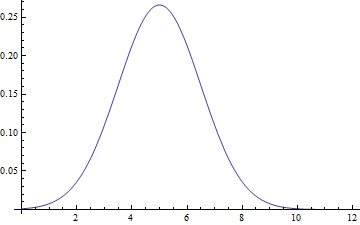
\includegraphics[width=\linewidth]{gp_1d.png}
  \caption{Univariate Gaussian}
  \label{fig:gaussian_1d}
\end{minipage}%
\begin{minipage}{.41\linewidth}
  \centering
  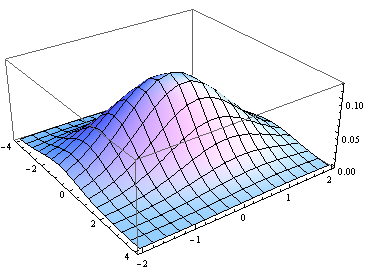
\includegraphics[width=\linewidth]{gp_2d.png}
  \caption{Multivariate Gaussian}
  \label{fig:gaussian_2d}
\end{minipage}

\label{fig:test}
\end{figure}


\subsection{Bayesian Probability Model}

The traditional linear regression method is rigid in terms of learning the parameters. It gives fixed values for parameters for one observed dataset. Therefore for every new observed datapoint, the parameters are bound to change. As always we only know numeric values of the parameters, it is hard to predict about how much they can change for the next ovserved data point.  It would be effective to learn a probability distribution over the parameters rather than fixed values. Having a distribution over parameters gives us space where the parameters can move, which is convenient to understand a stochastic process. Bayesian probability model starts with a prior distribution over parameters and changes the distribution based on observations.

Bayesian probability model is built after \textit{Bayes'} rule. It allows us to start with a prior belief on the data, which is an initial probability distribution associated to the data. Experiments generate evidences, which are used to change the prior belief, i.e. the initial distribution. The new distribution we get after incorporating the evidences is called posterior. The formulation is given below.

\subsubsection{Bayes' Rule}

We start with the expression of Bayes' rule. Say we have two random variables, $x$ and $y$, where $x$ is an independent variable but $y$ depends on $x$. The probability of $x$ is given by $p(x)$, the joint probability of $x$ and $y$ is given by $p(y, x)$. We can break $p(y, x)$ in $p(y|x)p(x)$ or $p(x|y)p(y)$ (Here $p(x|y)$ cannot be written as $p(x)$ if $x$ is conditionally dependant on $y$). Therefore,

\begin{eqnarray}
p(y, x) = p(y|x)p(x) = p(x|y)p(y)\nonumber\\
p(y|x) = \frac{p(x|y)p(y)}{p(x)}
\end{eqnarray}


The term $p(x)$ is marginalized over all possible values of $y$, so we can write $p(x)$ as,

\begin{equation}
p(x) = \sum_i{p(x|y_i)p(y_i)}
\end{equation}


Combining Eqn. \ref{reg_param} and Eqn. \ref{gauss_single_var_dist},

\begin{equation}
p(y|x) = \frac{p(x|y)p(y)}{\sum_i{p(x|y_i)p(y_i)}}
\end{equation}

In case $y$ is a continuous variable,

\begin{equation}
p(y|x) = \frac{p(x|y)p(y)}{\int_y{p(x|y)p(y)dy}}
\end{equation}

We start with the assumption that $y_i$ differs from $f(\mathbf{x}_i)$ because of noise, also Each noise term $\epsilon_i$ follows Gaussian i.i.d. $\mathcal{N}(0, \sigma ^2)$. Therefore the i\textsuperscript{th} can be written as,

\begin{eqnarray}
y_i = f(\mathbf{x}_i) + \epsilon_i \nonumber \\
y_i = \theta ^T \mathbf{x}_i + \epsilon_i && \text{where $\theta, \mathbf{x}_i \in \mathcal{R}^m$}
\end{eqnarray}

The PDF associated with $\epsilon_i$ is,

\begin{equation}
p(\epsilon_i) = \frac{1}{\sqrt{2 \pi} \sigma} exp(-\frac{\epsilon^2}{2 \sigma^2})
\end{equation}


It follows from Eqn. \ref{gauss_single_var_dist} that $(y_i - \theta ^T x_i) \sim \mathcal{N}(0, \sigma^2)$, so by combining Eqn. \ref{gauss_single_var_dist} and Eqn. \ref{gauss_single_var_sym},

\begin{equation}
p(y_i - \theta ^T x_i) = \frac{1}{\sqrt{2 \pi} \sigma} exp(-\frac{(y_i - \theta ^T x_i)^2}{2 \sigma^2})
\end{equation}

From Eqn. \ref{gauss_multi_var_dist} we conclude,

\begin{eqnarray}
\begin{split}
&p(y_i - \theta ^T \mathbf{x}_i) \sim \mathcal{N}(0, \sigma^2) \nonumber \\
&p(y_i | \mathbf{x}_i, \theta) \sim \mathcal{N}(\theta^T \mathbf{x}_i, \sigma^2)
\end{split}
\end{eqnarray}

We need to calculate the distribution over $\theta$ based on observed dataset $S = \{\mathbf{x}_i, y_i\}_{i=1}^n$ consisting of $n$ data points. The conditional PDF over $\theta$ given $S$ would be,

\begin{eqnarray}
\begin{split}
p(\theta | S) &= \frac{p(\theta)p(S | \theta)}{p(S)} \nonumber \\
&~\\
p(\theta | S) &= \frac{p(\theta)p(S | \theta)}{\int p(\theta)p(S | \theta)d\theta} \nonumber \\
&~\\
p(\theta | S) &= \frac{p(\theta) \prod_{i=1}^n p(y_i | \mathbf{x}_i, \theta)}{\int p(\theta) \prod_{i=1}^n p(y_i | \mathbf{x}_i, \theta) d\theta}
\end{split}
\end{eqnarray}

Now $y_*$, for the next unobserved data point $S_* = {y_*, x_*}$ for some $x_*$ given $S$, can be formulated as below,

\begin{equation}
p(y_* | x_*, S) = \int p(y_* | x_*, \theta)p(\theta | S)d \theta
\label{conti_rnd_var_bayes_poster}
\end{equation}

\subsection{Gaussian Process}

The problem with the multivariate Gaussian distribution is that we are confined to the number of operating variables or the dimension of the input $\mathbf{x_i} \in \mathcal{R}^m$. Therefore to calculate the posterior distribution for $y_*$, we had to go for a two step solution. Firstly we learned a multivariate Gaussian posterior $p(\theta | S)$ over the set of parameters $\theta \in \mathcal{R}^m$ and secondly used it to calculate the posterior over $y_*$.

It would be nice to have a mathematical framework that does not try to learn a finite set of parameters. Therefore it does not care about dimensions of input, thus truly represents an infinite dimensional multivariate Gaussian distribution. This representation is known as Gaussian process.

In our example of rainfall prediction, we consider $x_i \in \mathcal{R}$ to be summer temperature. Here the independent random variable $x_i$ is single dimensional. If we consider spring temperature also for that particular year then $x_i = \{x_i, x_j\} \in \mathcal{R}^2$ becomes two dimensional. No matter how many different temperatures we consider, $x_i \in \mathcal{R}^m$ remains a finite dimensional vector. Gaussian process helps in building a framework that actually allows us to fit any number of dimensions in. We do not have to fix $m$ beforehand. Therefore we can make $x_i$ represent various different temperatures at different months, weeks, days, hours and so forth.

Previously we showed different random variables over different co-ordinate axis to represent multivariate distribution. We cannot see beyond three dimensions, so to draw infinite dimensional distributions we do not represent one random variable on a single axis. For example $X$-axis does not represent any particular random variable in $x_i$ anymore, rather the entire $x_i$. As we can fit infinite number of points on $X$- axis, we can represent infinite dimensions on it. If $x_i$ is a three dimensional vector, we show three points on $X$-axis.

To represent the regression problem here, we have,

\begin{equation}
y_i = f(\mathbf{x}_i) + \epsilon_i
\label{reg_sym_noise}
\end{equation}

$\epsilon_i \sim (0, \sigma^2))$ is the standard Gaussian noise.

Without considering any parameter set, we try to learn the function $f$. We treat $f$ as a dependent random variable on $x_i$. A continuous function can represent infinite number of points on it. Therefore $f$ can fit over an infinite dimensional $x_i$. Thus Gaussian process gives us a multivariate distribution over functions.

\begin{figure}[h!]
\centering
\begin{minipage}{.5\linewidth}
  \centering
  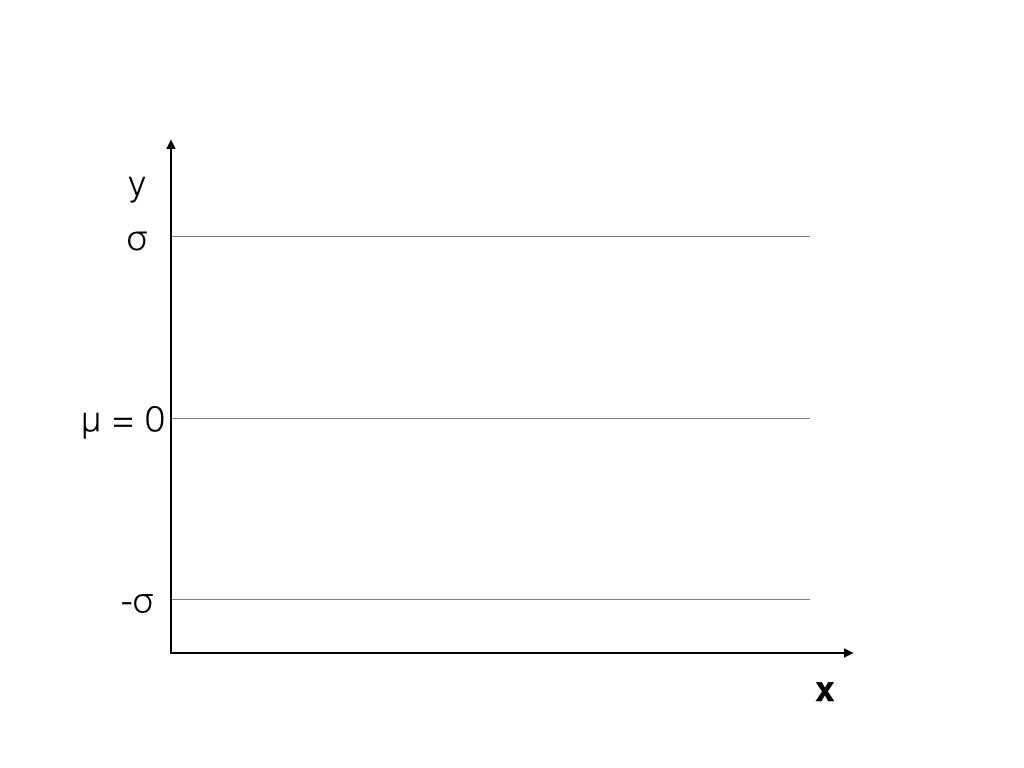
\includegraphics[width=\linewidth]{figures/GP_1.png}
  \caption{Prior with zero mean}
  \label{fig:sub1}
\end{minipage}%
\begin{minipage}{.5\linewidth}
  \centering
  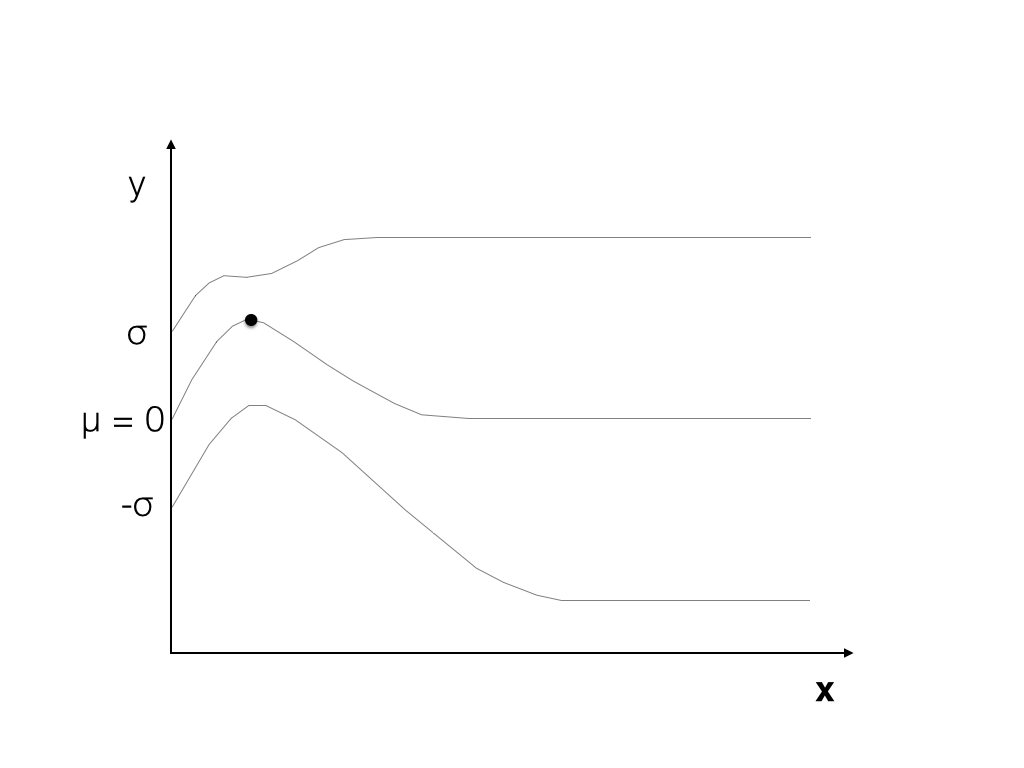
\includegraphics[width=\linewidth]{figures/GP_2.png}
  \caption{Posterior with one evidence}
  \label{fig:sub2}
\end{minipage}

\begin{minipage}{.5\linewidth}
  \centering
  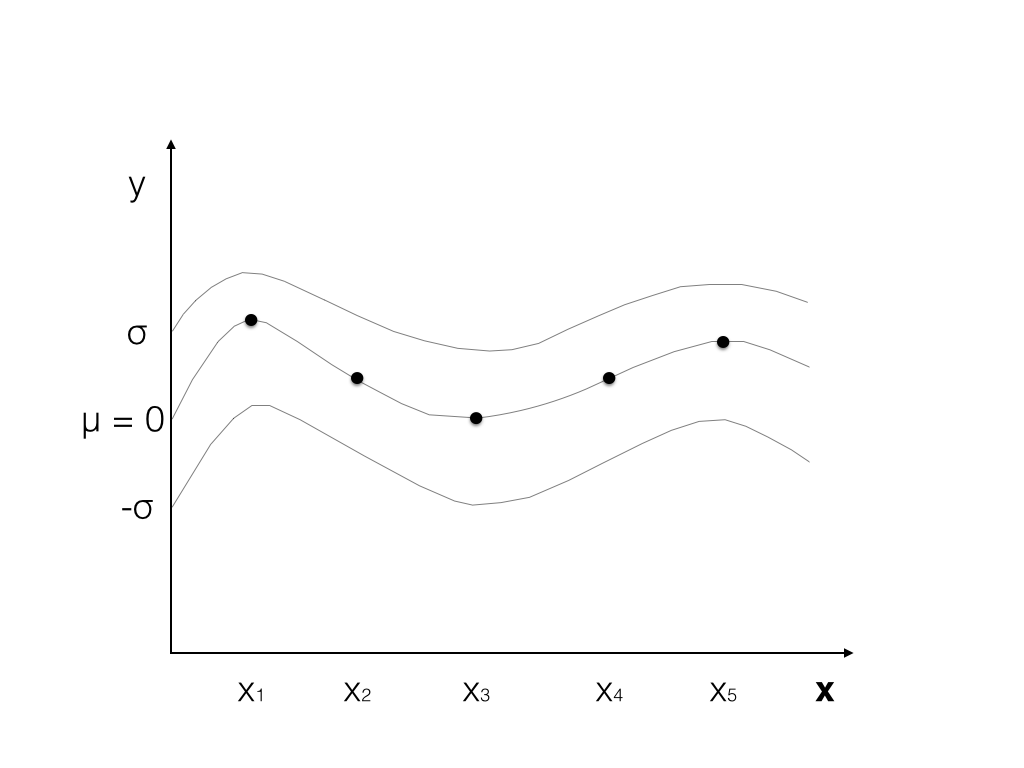
\includegraphics[width=\linewidth]{figures/GP_3.png}
  \caption{More evidences}
  \label{fig:sub1}
\end{minipage}%
\begin{minipage}{.5\linewidth}
  \centering
  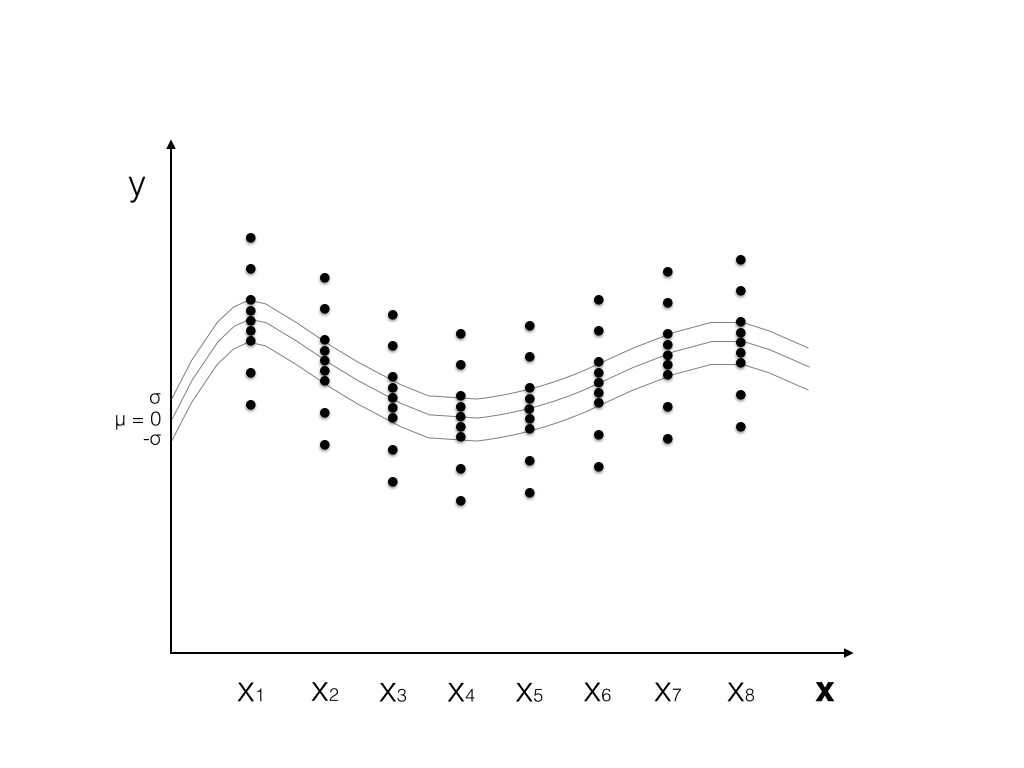
\includegraphics[width=\linewidth]{figures/GP_4.png}
  \caption{Learned function with entire training set}
  \label{fig:sub2}
\end{minipage}

\label{fig:test}
\end{figure}

Say, $\mathcal{F} = \{f_1, f_2, ..., f_n, f_{n+1}, ... \infty\}$ is a set of functions that can operate over $\mathbf{x}_i$. A function $f_1$ can take any form like $f_1(x) = (x + 2)$ or $f_1(x) = x^2$ or $f_1(x) = \exp(\sin(x)^5)$, as long as $f_1(x) \in \mathcal{R}$. From this infinite set $\mathcal{F}$, we need to find the proper $f$ that truly represents $y$.

To differentiate a function from a regular random variable we denote a function $f$ as $f(.)$ from now on. We start with a prior distribution over $\mathcal{F}$, given by,

\begin{equation}
f(.) \sim (m(.), k(.,.))
\end{equation}

The prior is shown in Figure 1 with zero mean. Before getting evidences, the prior distribution has uniform confidence interval around the mean for the entire space. Figure 2 shows that after getting one evidence point the space around that point shrinked. We exclude all the functions that do not pass through our evidence point. The mean function has to pass through that point, therefore it shifted and the confidence interval also narrowed down accordingly. Figure 3 shows the same effect for more evidence points. Figure 4 finally shows the shape of the posterior function when we have enough evidences.

As we are operating on a distribution over functions, the mean $m(.)$ and covariance matrix $k(.,.)$ are also functions. The domain of $f(.)$ is a vector $x_i \in \mathcal{R}^M$ where $M \to \infty$. $m(.)$ is the mean function which gives the mean of any random variable $x_{ip} (x_{ip} \in \mathbf{x}_i, p \in M)$,

$$
m(x_{ip}) = \mu_{ip}
$$

$k(.,.)$ takes two random variables, $x_{ip}$ and $x_{iq}$ and gives the covariance between them as,

$$
k(x_{ip}, x_{iq}) = Covariance(x_{ip}, x_{ip})
$$

$k(.,.)$ is also called the Kernel function.

To represent the multivariate distribution over functions operating over any finite subset $\mathbf{x}_i^m \in \mathbf{x}_i$ we can write in matrix form as,

$$
\begin{pmatrix}
f(x_1) \\
f(x_2) \\
\vdots \\
f(x_m)
\end{pmatrix}
\sim\left(%
\begin{pmatrix}
m(x_1) \\
m(x_2) \\
\vdots \\
m(x_m)
\end{pmatrix}
,%
\begin{pmatrix}
k(x_1, x_1) k(x_1, x_2) \hdots k(x_1, x_m) \\
k(x_2, x_1) k(x_2, x_2) \hdots k(x_2, x_m) \\
\vdots \\
k(x_m, x_1) k(x_m, x_2) \hdots k(x_m, x_m) 
\end{pmatrix}\right)
$$

Which can be written as,

\begin{equation}
f(\mathbf{x}_m) \sim (m(\mathbf{x}_m), K(\mathbf{x}_m))
\label{gauss_proc_multi_var_sym}
\end{equation}

We see how easy Gaussian process is to customize, any time we can extract a finite subset out of the infinite distribution.

To simplify the calculation, we start with a zero mean prior as,

\begin{equation}
f(.) \sim (0, k(.,.))
\label{gauss_proc_func_0_mean_sym}
\end{equation}

Combining Eqn. \ref{gauss_proc_multi_var_sym} and Eqn. \ref{gauss_proc_func_0_mean_sym} we get,

\begin{equation}
f(\mathbf{x}_m) \sim (0, K(\mathbf{x}_m))
\end{equation}

We take $\mathbf{x}_m$ as training set, so we have observed $\mathbf{y}_m$. Say we have another finite subset $\mathbf{x}_m^*$, which is the test set. We need to predict outputs $\mathbf{y}_m^*$ for $\mathbf{x}_m^*$. Both the subsets came from the same infinite Gaussian distribution. So for $\mathbf{x}_m^*$ we write,

\begin{equation}
f(\mathbf{x}_m^*) \sim (0, K(\mathbf{x}_m^*))
\end{equation}

We combine Eqn. \ref{conti_rnd_var_bayes_poster} and Eqn. \ref{reg_sym_noise} together as,

\begin{equation}
\begin{pmatrix}
f(\mathbf{x}_m) \\
f(\mathbf{x}_m^*)
\end{pmatrix}
\sim \left( %
0, %
\begin{pmatrix}
K(\mathbf{x}_m, \mathbf{x}_m) & K(\mathbf{x}_m, \mathbf{x}_m^*) \\
K(\mathbf{x}_m^*, \mathbf{x}_m) & K(\mathbf{x}_m^*, \mathbf{x}_m^*)
\end{pmatrix}\right)
\end{equation}

We also have noise vectors $\mathbf{\varepsilon} \in \mathcal{R}^m$ and $\mathbf{\varepsilon^*} \in \mathcal{R}^m$. We get the distribution over $\mathbf{y}$ by adding noise to the distribution over $f(.)$. Addition of multiple Gaussians remains Gaussian, so we can write,

\begin{eqnarray}
\begin{pmatrix}
\mathbf{y}_m \\
\mathbf{y}_m^*
\end{pmatrix}
= %
\begin{pmatrix}
f(\mathbf{x}_m) \\
f(\mathbf{x}_m^*)
\end{pmatrix}
+%
\begin{pmatrix}
\mathbf{\varepsilon} \\
\mathbf{\varepsilon^*}
\end{pmatrix}
\sim \left( %
0, %
\begin{pmatrix}
K(\mathbf{x}_m, \mathbf{x}_m) + \sigma^2 \mathbf{I} & K(\mathbf{x}_m, \mathbf{x}_m^*) \\
K(\mathbf{x}_m^*, \mathbf{x}_m) & K(\mathbf{x}_m^*, \mathbf{x}_m^*) + \sigma^2 \mathbf{I}
\end{pmatrix}\right) \nonumber \\
\left.
\begin{pmatrix}
\mathbf{y} \\
\mathbf{y}^*
\end{pmatrix}
\right\vert_{\mathbf{x}_m, \mathbf{x}_m^*}
= %
\begin{pmatrix}
f(.) \\
f(.)^*
\end{pmatrix}
+%
\begin{pmatrix}
\mathbf{\varepsilon} \\
\mathbf{\varepsilon^*}
\end{pmatrix}
\sim \left( %
0, %
\begin{pmatrix}
K(\mathbf{x}_m, \mathbf{x}_m) + \sigma^2 \mathbf{I} & K(\mathbf{x}_m, \mathbf{x}_m^*) \\
K(\mathbf{x}_m^*, \mathbf{x}_m) & K(\mathbf{x}_m^*, \mathbf{x}_m^*) + \sigma^2 \mathbf{I}
\end{pmatrix}\right)
\end{eqnarray}

Using Bayesian posterior calculation it can be shown that,

\begin{equation}
\mathbf{y_m}^* | \mathbf{y_m}, \mathbf{x}_m, \mathbf{x}_m^* \sim (\mu^*, \Sigma^*)
\end{equation}

This is the function represented by Figure 4.

where,

\begin{equation}
\mu^* = K(\mathbf{x}_m^*, \mathbf{x}_m)(K(\mathbf{x}_m, \mathbf{x}_m) + \sigma^2 \mathbf{I})^{-1}\mathbf{y_m}
\label{gauss_poster_mean}
\end{equation}

and,

\begin{equation}
\Sigma^* = K(\mathbf{x}_m^*, \mathbf{x}_m^*) + \sigma^2 \mathbf{I} - K(\mathbf{x}_m^*, \mathbf{x}_m)(K(\mathbf{x}_m, \mathbf{x}_m) + \sigma^2 \mathbf{I})^{-1} K(\mathbf{x}_m, \mathbf{x}_m^*)
\label{gauss_poster_var}
\end{equation}


\subsubsection{Applying Gaussian Process to Bandit Problems}

We ended \ref{sec:UCB} by mentioning that upper confidence bound works well in finite action spaces. Here we will see how gaussian process helps us is determining upper confidence bound in infinitly large action spaces, where estimating mean for each action distribution is practically impossible. We represent the actions $A$ as our input space as before and we want to learn a function that gives mean rewards $\mu_{a_i}$ for each $a_i$. Theoretically the more $a_i$s we explore, the closer we get to the actual reward function. But in real life experiments it is not always possible to try all or nearly all the actions from a very large action space.
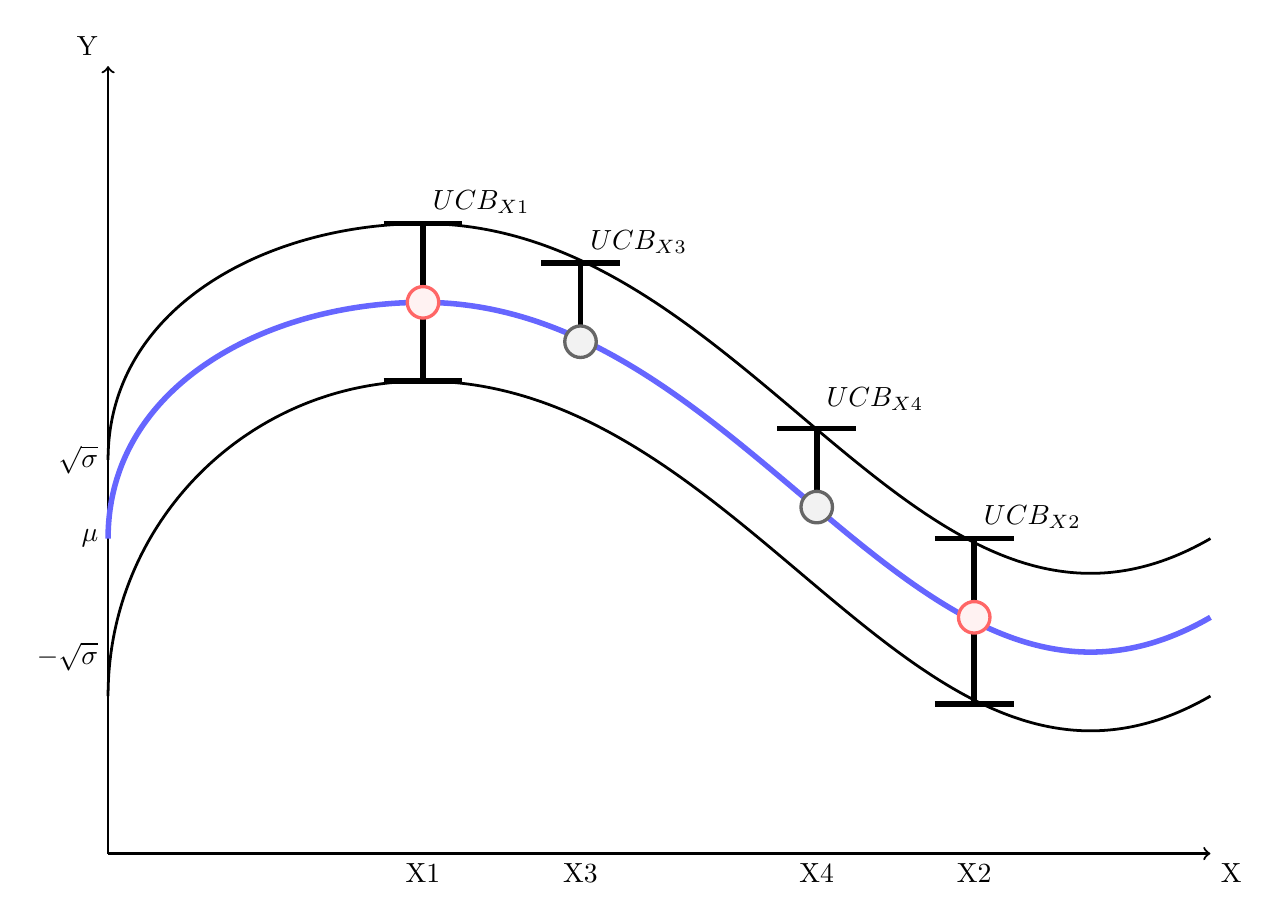
\begin{tikzpicture}


% Draw Axis

\draw[thick,->] (0,0) -- (14,0) node[anchor=north west]{X};
\draw[thick,->] (0,0) -- (0,10) node[anchor=south east]{Y};

% Draw Mean function
\draw[color=blue!60, line width=2pt] (0,4) to [out=90, in=180] (4,7)
to [out=0, in=210] (14,3);

% Draw Lower Bound (-var) function

\draw[line width=1pt] (0,2) to [out=90, in=180] (4,6)
to [out=0, in=210] (14,2);

% Draw Upper Bound (+var) function

\draw[line width=1pt] (0,5) to [out=90, in=180] (4,8)
to [out=0, in=210] (14,4);

% Draw Confidence Interval for X1

\draw[line width = 2pt] (4,6) -- (4,8);

\draw[line width = 2pt] (3.5,6) -- (4.5,6);

\draw[line width = 2pt] (3.5,8) -- (4.5,8);

% Draw X1

\filldraw[color=red!60, fill=red!5, very thick] (4,7) circle (0.2cm);

% Draw Confidence Interval for X2

\draw[line width = 2pt] (11,1.9) -- (11,4);

\draw[line width = 2pt] (10.5,1.9) -- (11.5,1.9);

\draw[line width = 2pt] (10.5,4) -- (11.5,4);

% Draw X4

\filldraw[color=red!60, fill=red!5, very thick] (11,3) circle (0.2cm);

% Draw dashed Confidence Interval for X3

\draw[line width = 2pt] (6,6.5) -- (6,7.5);

\draw[line width = 2pt] (5.5,7.5) -- (6.5,7.5);

% Draw X3

\filldraw[color=black!60, fill=black!5, very thick] (6,6.5) circle (0.2cm);

% Draw dashed Confidence Interval for X4

\draw[line width = 2pt] (9,4.4) -- (9,5.4);

\draw[line width = 2pt] (8.5,5.4) -- (9.5,5.4);

% Draw X4

\filldraw[color=black!60, fill=black!5, very thick] (9,4.4) circle (0.2cm);

% Draw Labels on X-Axis

\node [below] at (4,0) {X1};

\node [below] at (11,0) {X2};

\node [below] at (6,0) {X3};

\node [below] at (9,0) {X4};

% Draw Labels on Y-Axis

\node [left] at (0,4) {$\mu$};

\node [left] at (0,2.5) {$-\sqrt{\sigma}$};

\node [left] at (0,5) {$\sqrt{\sigma}$};

% Draw UCB Labels

\node [above right] at (4,8) {$UCB_{X1}$};

\node [above right] at (11,4) {$UCB_{X2}$};

\node [above right] at (6,7.5) {$UCB_{X3}$};

\node [above right] at (9,5.5) {$UCB_{X4}$};

\end{tikzpicture}
By carefully observing how the posterior of the reward function changes given the ovservations so far and then choosing the next action, we can nearly estimate the actual reward function very quickly. This requires some optimization over selection of actions which is beyond the scope of this discussion. Also the more we select each action, by the \textit{law of large numbers}, the closer we go to the actual mean reward associated with that action.

Next we will see how we modelled our system based on these discussion. But before that we will get an overview of other CBIR systems present.

\section{Related Works}

We had many content based image retrieval systems so far over the past few years. These include Query By Image Content (QBIC) by IBM \cite{QBIC}, Photobook by MIT \cite{Photobook}, Virage by Virage Technologies \cite{Virage}, PicSOM \cite{PicSOM} and Pinview \cite{Pinview}. We will discuss PicSOM and Pinview briefly.

\subsection{PicSOM}

PicSOM is a recent CBIR system that uses large unannotated image databases. It is the first system in its genre that uses \textit{Self Organizing Maps}(SOM) \cite{SOM}, especially it uses tree structured SOM (TS-SOM) \cite{TSSOM} \cite{TSSOM_progress}. The system can be configured to use with multiple image databases and it can handle multiple features. New features can also be introduced to the system as long as the feature can be represented in fixed dimensions and Euclidean metric can be applied to measure the distances between images. The system uses five different features namely, Average Colour, Colour Moments, Texture Neighbourhood, Shape Histogram and Shape FFT. For each of these features the system calculates the corresponding TS-SOM. The TS-SOMs are trained in a top-to-bottom manner by presenting the extracted feature vectors for each image to the corresponding TS-SOM multiple times. After the training, each node in the TS-SOM contains a model vector which roughly averages all the feature vectors mapped to that node down below. Also if the training is proper, each node at the bottom of a TS-SOM should uniquely represent one single image.

PicSOM is a web application and it starts with providing a choice of the image database to the user. Once the user selects the database, it shows a few images from that database to the user. The user selects a subset of the images from the shown set and continues. This subset is passed as a query to the system. The feature vectors for respective features for images from the selected subset are calculated and passed to the TS-SOMS to find out similar images. Different TS-SOMs will give different images as a result of similarity measure. Somwhow the results need to be combined or only the TS-SOM, whose feature best represents the user's intention in the selection, have to be used. The user could have been given a choice regarding which feature he wants to use for the current search. But features are not very straight forward always. For example if the user is a layman, he might not be aware about Shape-FFT. Therefore it is better if the system decides which feature would perform better by observing the selected subset. PicSOM has a very good solution to this problem. It passes the feature vectors for selected images to all the TS-SOMs and observes the spread of the images. The TS-SOM that represents the selected images the closest to each other or the least scattered, has the best performing feature for the current search.

The images in the selected subset are marked as positive and the images ignored by the user are marked as negative. The system uses a low pass filter mask to convolve the TS-SOM. This way the positive effect of the nodes, mainly associated with images marked so, are conveyed to the neighbouring nodes. In the next iteration, images from nodes with high positive values are selected and shown to the user and the process continues.

\subsection{Pinview}

Pinview uses PicSOM engine internally. It incorporates multiple input modalities for accepting relevance feedback namely click and eye movement. It uses multi-armed bandit algorithm, \textit{Linrel} \cite{linrel}, to calculate relevance score of an image as a linear combination of feature vectors of previously shown images. Say at iteration $t$, the feature vectors of all shown images over the past $t-1$ iterations is represented by the matrix of row vectors of features of images $\mathbf{X}_t = \{\mathbf{x}_1, ..., \mathbf{x}_{t-1}\}$. The collected relevance score so far is given by column vecror $y_t = \{y_1, ..., y_{t-1}\}$. The algorithm calculates an optimal weight vector $\hat{\mathbf{w_t}}$ such that,

$$
y_t = \mathbf{X}_t . \hat{\mathbf{w_t}}
$$

After calculating $\hat{\mathbf{w_t}}$, for each new image $x_i \notin \mathbf{X}_t$, which has not been presented to the user so far, is given a relevance score calculated by,

$$
y_i = x_i . \hat{\mathbf{w_t}}
$$

Once the relevance score is estimated, the system computes the upper confidence bound of that relevance as $y_i + k \sigma_i$ and the image with the largest upper confidence value is presented next. Here $k$ is a constant that controls the exploration.

PicSOM selects the best performing image feature by examining the adjacency of selected images on TS-SOMs. But sometimes it is really required to combine features. Colour might work well on a query where the user is searching for blue skies, but to search blue sky with cloud formation, colour and texture together might play better. Therefore sometimes it is required to combine various kernels of different features. Pinview does the same by \textit{multiple kernel learning} (MKL) \cite{mkl}. If there are $n$ different kernels, $K = \{k_1, k_2, ..., k_n\}$, for any two images $i, j$, the combined kernel function \cite{Pinview} would be,

$$
k_{\eta}(i, j) = \sum_{i=1}^n \eta_i k_i(i, j)
$$

Here $\eta = \{\eta_1, ...\eta_n\}$ are the weights given to kernel functions.

\section{System description}

We have developed a small CBIR system, modelled over reinforcement learning, especially bandit problems. The system uses relevance feedback from users as immediate rewards in each step. We start with a set of images, assuming each of them having an equal prior probability to get selected. A few of them are shown to the user and relevance feedback is collected. These images, shown to the user, along with their acquired relevance feedback, are fed to the gaussian process regression framework to calculate the posterior probability on each image not shown so far. UCB for each of these images are then calculated by adding the posterior mean and the positive standard deviation as discussed before. The image with largest UCB value is picked to be shown next.

\begin{figure}[h!]
  \centering
    \includegraphics[width=1.0\textwidth]{figures/Imse_System_Diagram}
    \caption{System diagram with hierarchical GP}
    \label{system_diagram_1}
\end{figure}

Bandit algorithms are designed to make one prediction at a time and each prediction takes the immediate reward received by the previous prediction into account. To select a set of images each iteration, we need to run the algorithm a few times but as before showing an image to the user, we do not have the relevance score for it ready, we use pseudo feedback to pick up the next image. This pseudo feedback is nothing but the posterior mean for the corresponding image. Once we select the desired number of images, we show them to the user, receive relevance feedback on them, replace the pseudo feedbacks with the actual feedbacks given by our user. This way we nullify the long term effect of pseudo feedbacks in our system.

We need to process the images before starting the actual experiments. Therefore we break the operation on the images into two parts as described below.

\subsection{Offline step}

\subsubsection{Feature extraction}

We have used MIRFLICKR 25000 \cite{mirflickr} image set for the experiment. \textcolor{red}{We are considering colour as the only feature. We extract histogram from each image and divide that into 512 sections and normalize, resulting a 512 dimensional vector. Thus each image is represented by a colour feature vector of dimension 512. Numerically each vector is a collection of 512 floating point numbers. (needs revision)}

\subsubsection{Kernel calculation}

We use "Cityblock" or "Manhattan" distance to calculate pairwise distance between two images, to feature vectors precisely. The distance is normalized by the number of dimensions i.e. 512. Therefore the number of dimensions are used as the length scale hyperparameter for the kernel. For any two images $x_i$ and $x_j$, the kernel function is,

\begin{equation}
K(x_i, x_j) = \sum_{l = 1}^{512}\frac{(|x_i^l - y_i^l|)} {512}
\end{equation}

Here $x_i^l$ and $y_i^l$ represent the $l$th dimensional value in the corresponding feature vectors of images $x_i$ and $y_i$ respectively.


We calculate all the pairwise distances among the 25000 images and build a $(25000 X 25000)$ distance matrix. This matrix serves as the entire co-variance matrix.

\subsubsection{Clustering images}

As we have a huge number of images, calculating UCB values for nearly all of them would be severely time consuming in each iteration. We can avoid so for very distant images. We apply K-means \cite{k_means} clustering algorithm to cluster images as mentioned by \cite{hierarchical_gp}. Each cluster centroid is the average of all the feature vectors associated to it. To select an image, we first calculate the UCB values for the cluster centroids and select the nearest one. Then we calculate UCB values for images only in that cluster and find out the nearest image.

\subsection{The online step}

We assign search tasks to users, say to find a suitable "red rose". The experiment starts by showing a set of random images to the user. The user finds one or more suitable images inside that set (there might not be one, we will discuss that later) and provides relevance feedback. The algorithm collects the shown image set and given relevance feedbacks and runs several times, as discussed earlier, to come up with the next set of suitable images. The iteration continues and as soon as the user finds the most desired image or several very much desired images he has in mind, the experiment ends.

Say, upto $t$ iterations, we showed $X_t = \{x_1, x_2, ..., x_t\}$ images and received relevance feedback $Y_t = \{y_1, y_2, ..., y_t\}$.

According to Eqn. \ref{gauss_poster_mean}, for the rest of the images, the posterior mean function would be,

\begin{equation}
\mu(x) = K(x, X_t)[K(X_t, X_t) + \sigma_{noise}^2I]^{-1}Y_t
\end{equation}

and, according to Eqn. \ref{gauss_poster_var}, the posterior co-variance function would be,

\begin{equation}
\sigma^2(x) = [K(x, x) + \sigma_{noise}^2I] - K(x, X_t)[K(X_t, X_t) + \sigma_{noise}^2I]^{-1}K(x, X_t)^T
\end{equation}

At $t+1$ iteration, image $x_{t+1}$ would be selected, satisfying,

\begin{equation}
x_{t+1} = argmax_x(\mu(x) + \beta\sqrt{\sigma^2(x)})
\end{equation}

We saw in Gaussian process discussion that after observing a significant amount of datapoints, the posterior variance becomes very small. Therefore the UCB value merely reflects the posterior mean, leading to an almost zero exploration. To keep the exploration alive, $\beta$ is introduced, which is a fraction that grows with discrete time or iterations. At any iteration $t$, $\beta = \sqrt{\log t}$.

\section{Experiments}

\subsection{Tasks}

The aim of these experiments were to study 1) how good exploration-exploitation strategy performs compared to mere exploitative method, 2) applicability of exploration based search in image retrieval in general. We designed three different categories of tasks for users. They are,

\begin{enumerate}
  \item Target search - Look for a specific image
  \item Category search - Look for a category
  \item Open ended search - Find a story, i.e. a set of images that gives a theme for an essay or an article
\end{enumerate}

\textit{Target search} was the most restrictive search, requiring an user to find out an image say a blue car.

\textit{Category search} was a bit broader, say to find a cat.

\textit{Open ended search} was the most broad one where the user was given no specific image to search for but a topic or theme like a visit to paris, out of which several image could be listed for an article on the same.

Each of these searches had three separate sub tasks as follows,

\textbf{for Target search}

\begin{enumerate}
  \item Red rose
  \item City by night
  \item Tall building
\end{enumerate}

\textbf{for Category search}

\begin{enumerate}
  \item Fruit
  \item Sunset
  \item Seashore
\end{enumerate}

\textbf{for Open ended search}

\begin{enumerate}
  \item A trip to africa
  \item Architecture
  \item Gardening
\end{enumerate}

Therefore we had nine separate search tasks altogether. An user had to go for all these searches but the order was different for each user.

\subsection{Participants and task allocation}

We recruited twenty postgraduate students from university as participants. Before the actual experiments, we provided a short training to them on the search interface. Each participant was instructed to finish a search task whenever they had felt done i.e. "red rose" is found or enough images gathered for writing an essay on "gerdening". The participants were allowed to go for 25 iterations maximum even if they had not found suitable images.

As mentioned earlier, the goal of this study was to find out how well our algorithm performs over pure exploitation. For the sake of completeness, we also had one algorithm for random selection of images. This algorithm is the simplest, which does nothing but selects images randomly without taking relevance feedback into consideration. Therefore we compared three different algorithms, Gaussian process upper confidence bound(GPUCB), Exploitation(EXPLOIT) and Random(RAND).

For each participant, the three subtask for each major task (target, category or open-ended) were a permutation of GPUCB, EXPLOIT and RAND. We also assigned random permutations of target, category and open-ended searches to different participants, so that they could not infer what is coming next.

The participants did not know about what algorithm had been used behind each task they performed.

In total we had 20 participants, each running a separate experiment out of a randomly permuted set of 9 search tasks. All the interactions were recorded.

\section{Results}

We studied mainly two things, firstly, how quickly i.e. in how many less iterations, GPUCB can finish compared two the EXPLOIT and RAND. Secondly, how many images gets positive feedback on average in GPUCB compared to EXPLOIT and RAND.

\begin{figure}[h!]
  \centering
    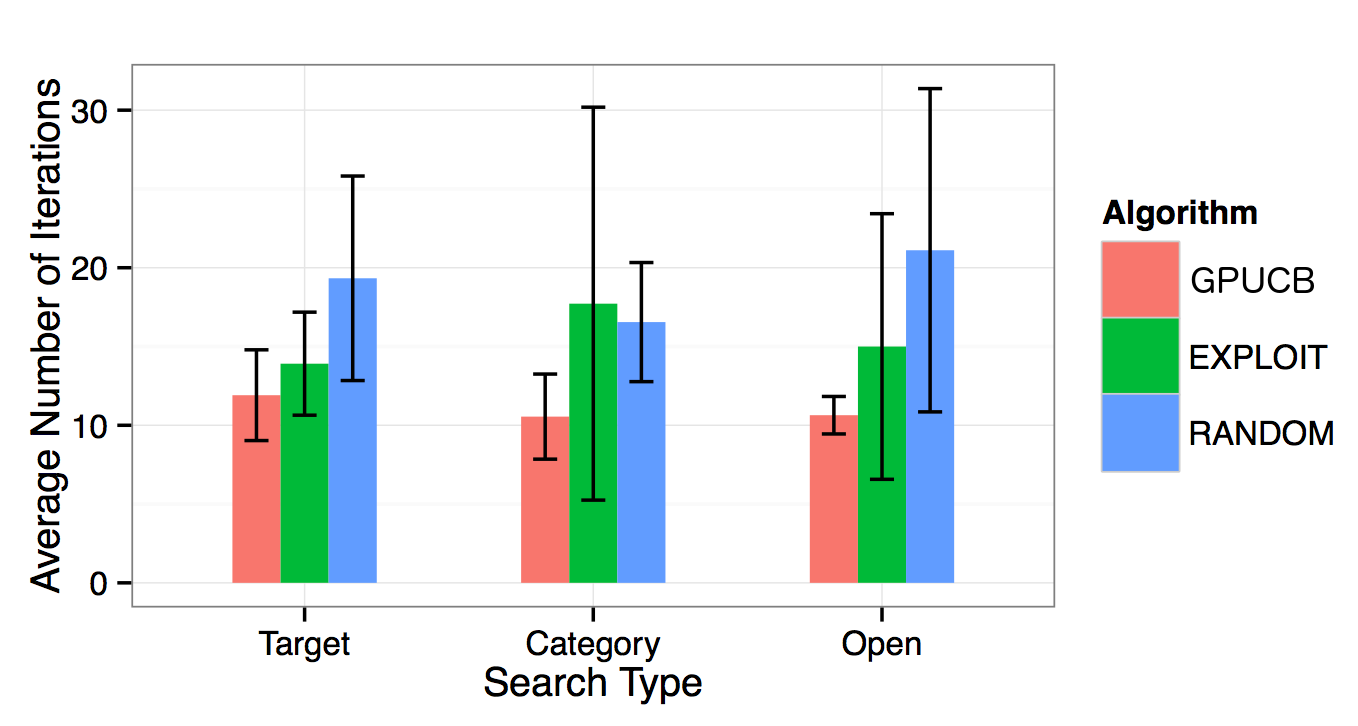
\includegraphics[width=1.0\textwidth]{figures/conf_intr.png}
    \caption{Average number of iterations along with 95\% confidence intervals to complete each type of search with GP-SOM, EXPLOIT and RAND systems.}
    \label{bar_chart}
\end{figure}

Figure \ref{bar_chart} clearly shows that GPUCB outperforms EXPLOIT and RAND in terms of average iterations needed to finish. In all the three major tasks, GPUCB could satisfy users in minimum number of iterations. Moreover, the confidence interval was consistent and small in case of GPUCB, while for EXPLOIT and RAND we see huge confidence interval leading to uncontrolled explorations.

EXPLOIT performed considerably better, almost as good as GPUCB, in target search. This is normal because in target search we specify fixed target, say "a red rose" to the user. If in the first iteration the user gets a red rose and provides maximum feedback possible to it, pure exploitation is the best way to conclude quickly rather than exploring, producing irrelevant images which will never receive feedbacks. Therefore GPUCB might not be the best option in target search. Category and open ended searches do not have fixed targets, thus require more exploration and GPUCB performed better than EXPLOIT in those cases as seen from Figure \ref{bar_chart}.

\begin{figure}[h!]
  \centering
    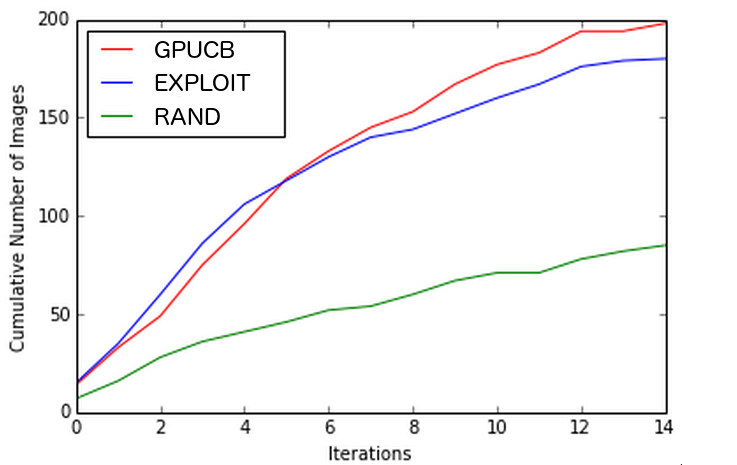
\includegraphics[width=0.32\textwidth]{figures/Target_Positive.png}
    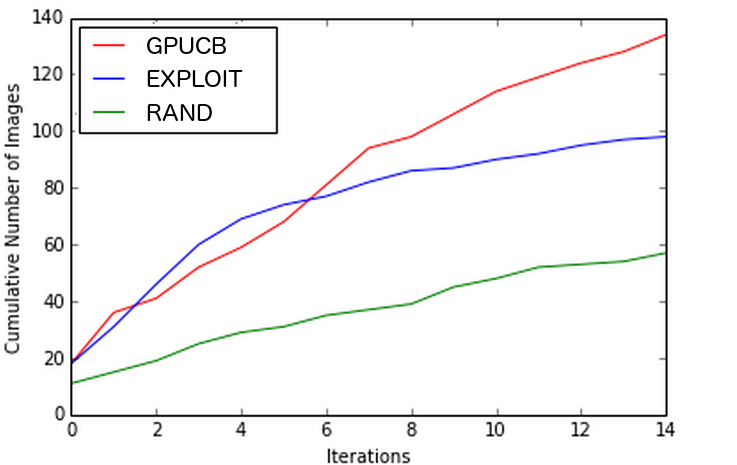
\includegraphics[width=0.32\textwidth]{figures/Category_Positive.png}
    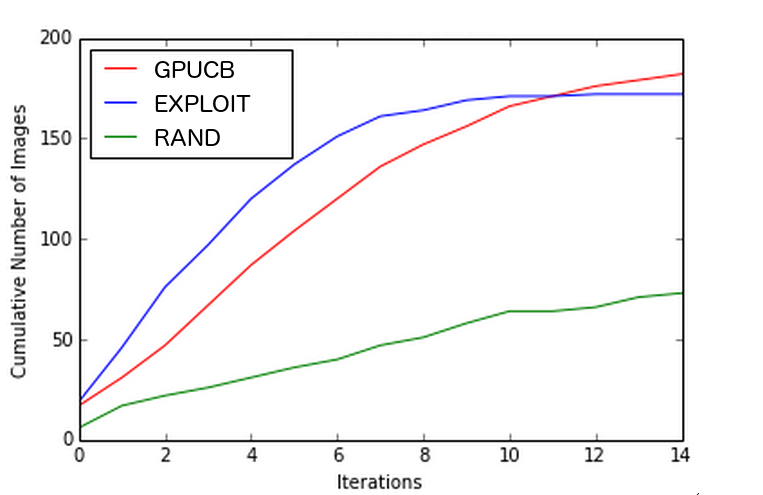
\includegraphics[width=0.32\textwidth]{figures/Open_Positive.png}
    \caption{Cumulative number of images marked as positive by user over iterations for GP-SOM, EXPLOIT and RAND for different type of searches}
    \label{positive_feedback}
\end{figure}

Figure \ref{positive_feedback} shows the cumulative number of images getting positive feedback over the three tasks in all three algorithms. We are using unannotated or untagged images, therefore the number of positive feedback over iterations are the only measure of how relevant the images were, presented to the user. As mentioned before, exploration did not affect target search to a great extent, so GPUCB and EXPLOIT generated more or less equal number of positive images. Both in category search and open ended search, GPUCB generated more positive feedback than the other two. In all three tasks, EXPLOIT started producing more positive feedbacks in the initial iterations, as GPUCB produced some irrelevant images due to exploration, but in the end fell behind GPUCB. GPUCB performed well to finish around twenty iterations in target search and fifteen in open ended search. The other two continued. RAND was clearly outperformed by the other two everywhere.

Here we will show the images shown per iteration, up to five iterations, for  two cases, Red Rose and City by Night, to show how well GPUCB performed and how more relevant images appeared with iterations. Red rose is shown from Figure \ref{red_rose_1} to \ref{red_rose_5}.

\begin{figure}[!h]
  \centering
    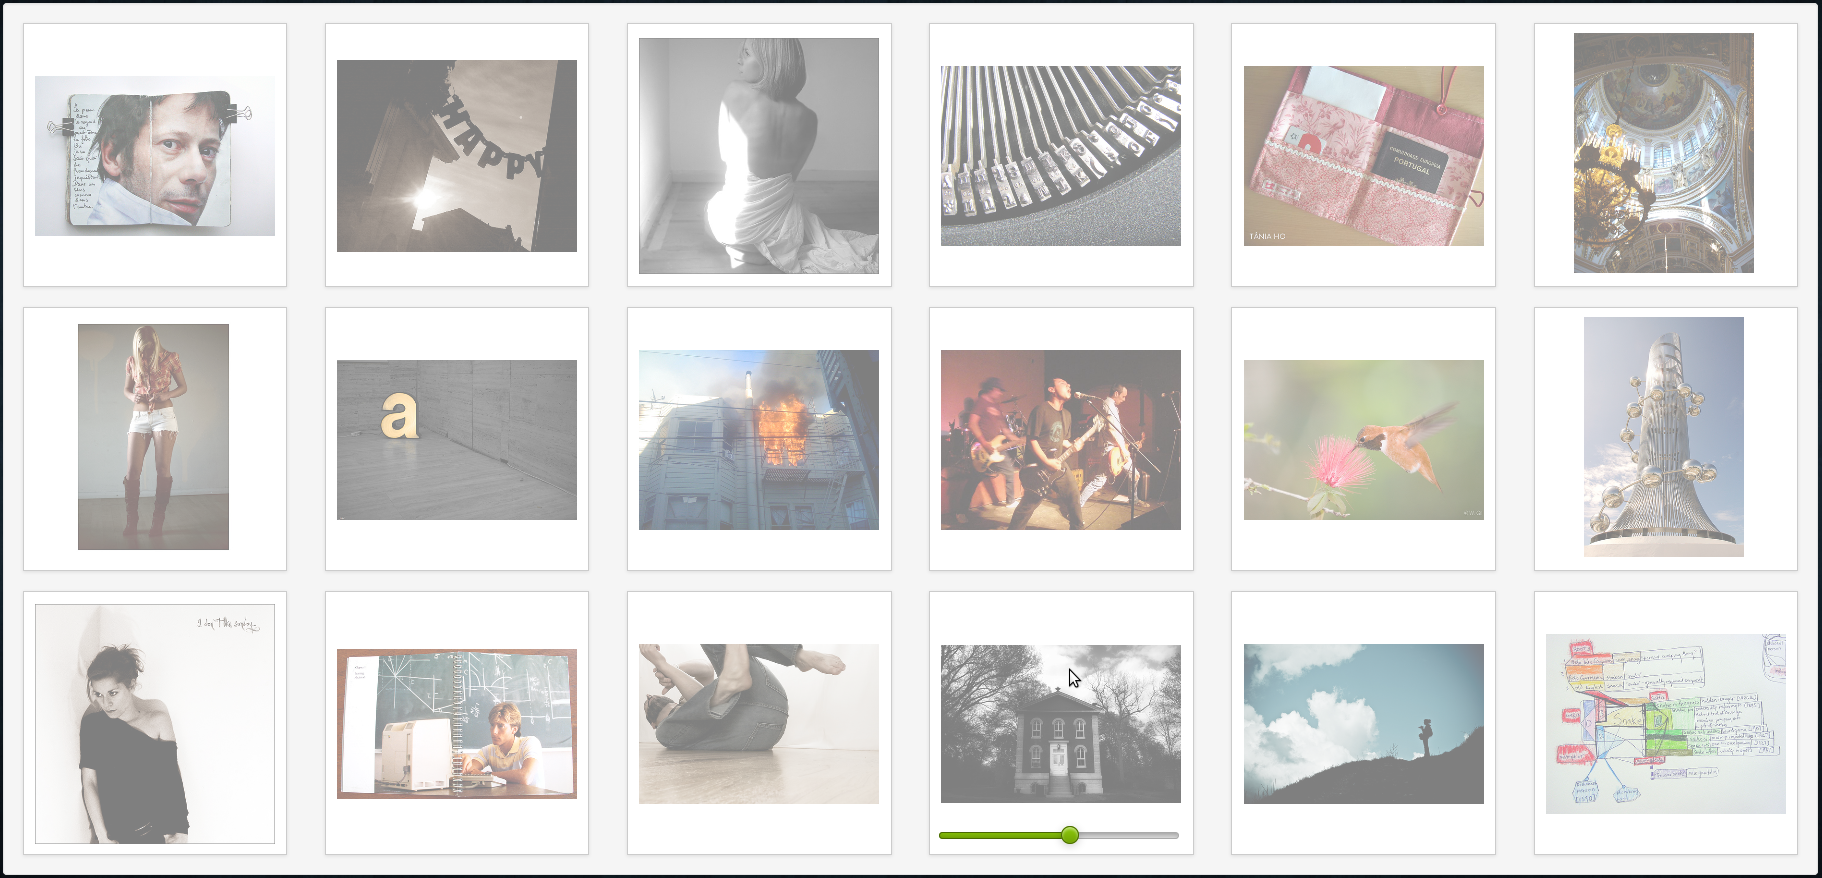
\includegraphics[width=0.90\textwidth,height=6cm]{figures/Rose_1.png}
    \caption{Red Rose Iteration 1}
    \label{red_rose_1}
\end{figure}

\begin{figure}[h!]
  \centering
    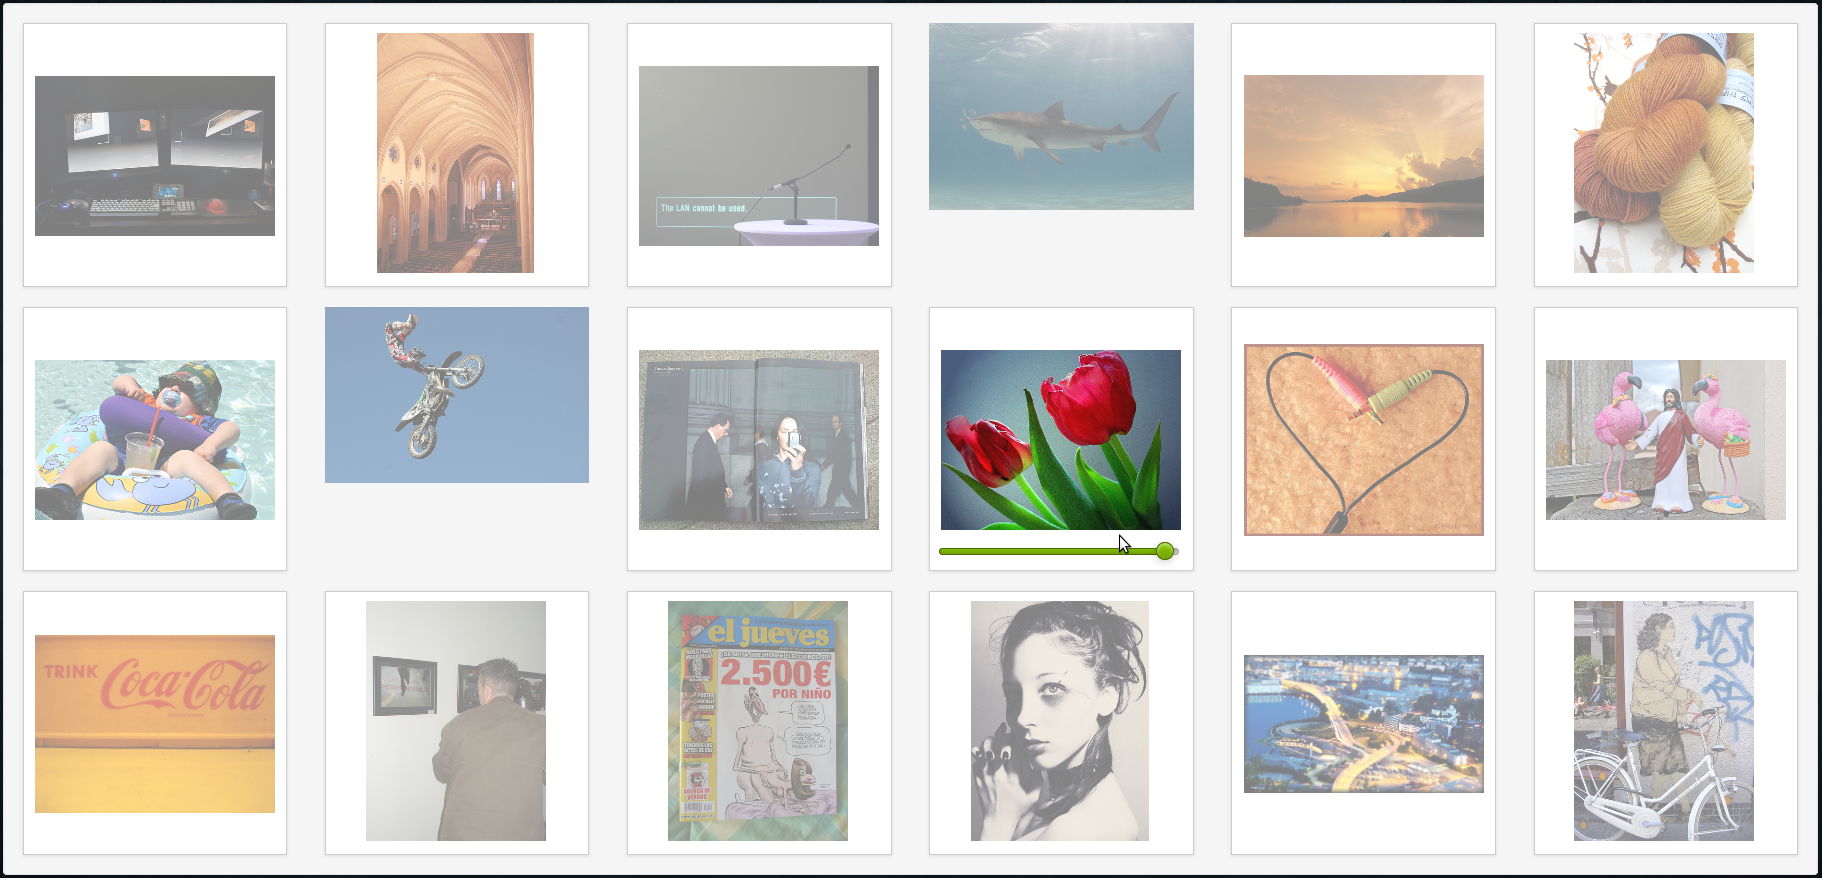
\includegraphics[width=0.90\textwidth,height=6cm]{figures/Rose_2.png}
    \caption{Red Rose Iteration 2}
    \label{red_rose_2}
\end{figure}

\begin{figure}[h!]
  \centering
    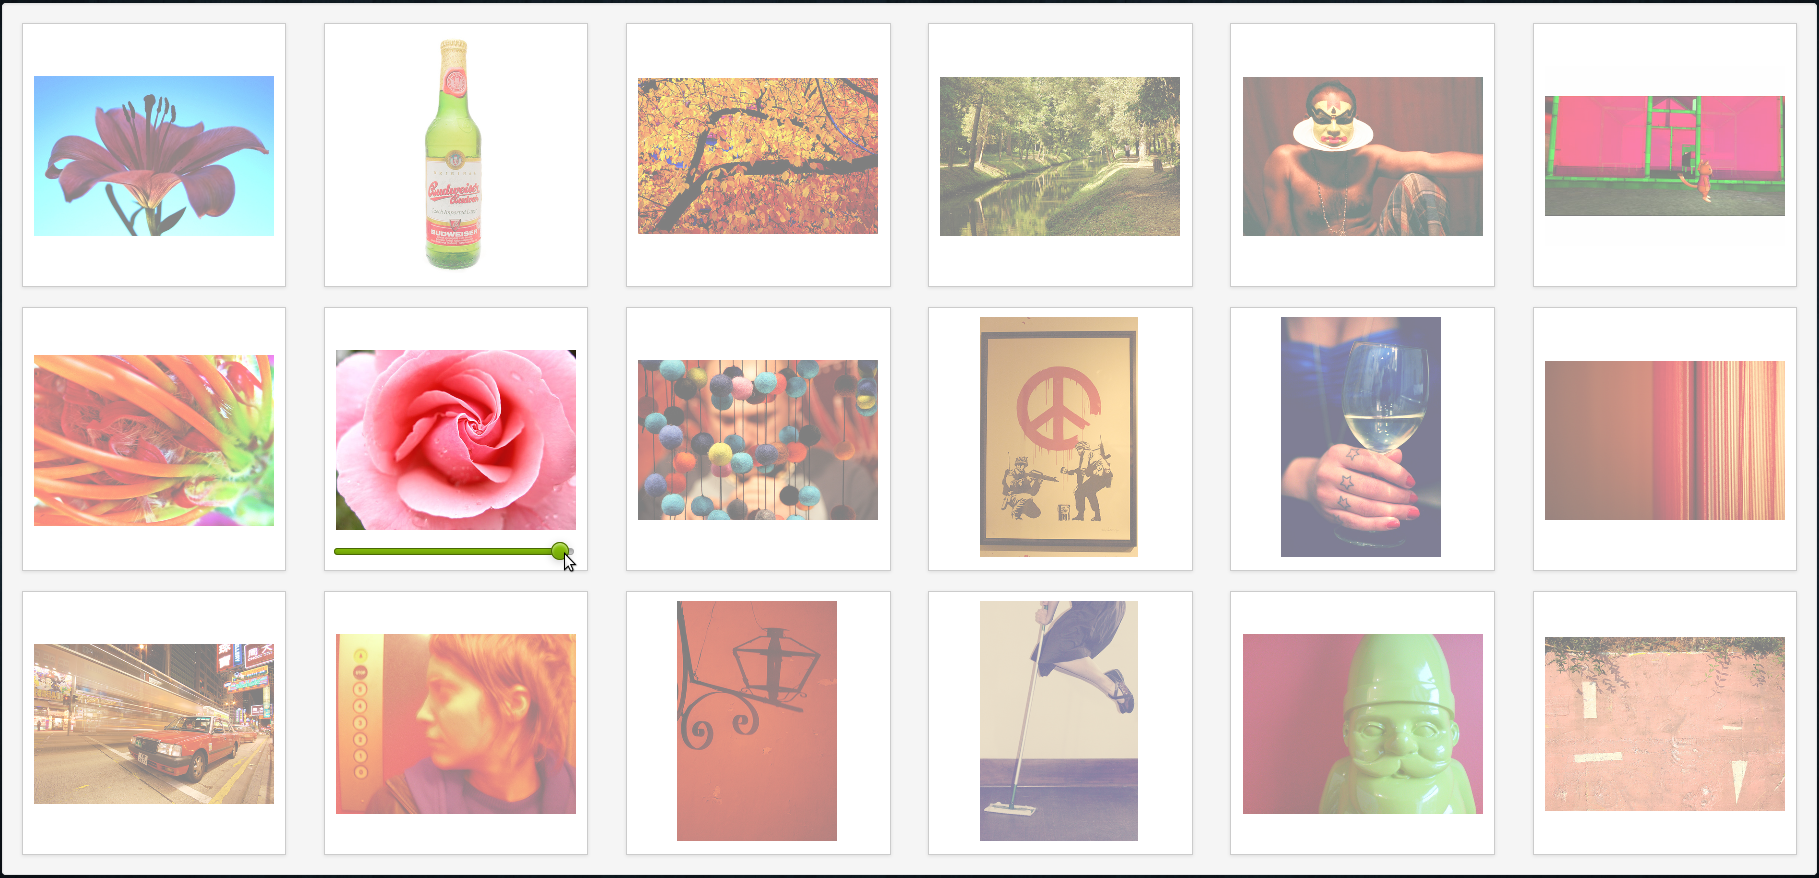
\includegraphics[width=0.90\textwidth,height=6cm]{figures/Rose_3.png}
    \caption{Red Rose Iteration 3}
    \label{red_rose_3}
\end{figure}

\begin{figure}[h!]
  \centering
    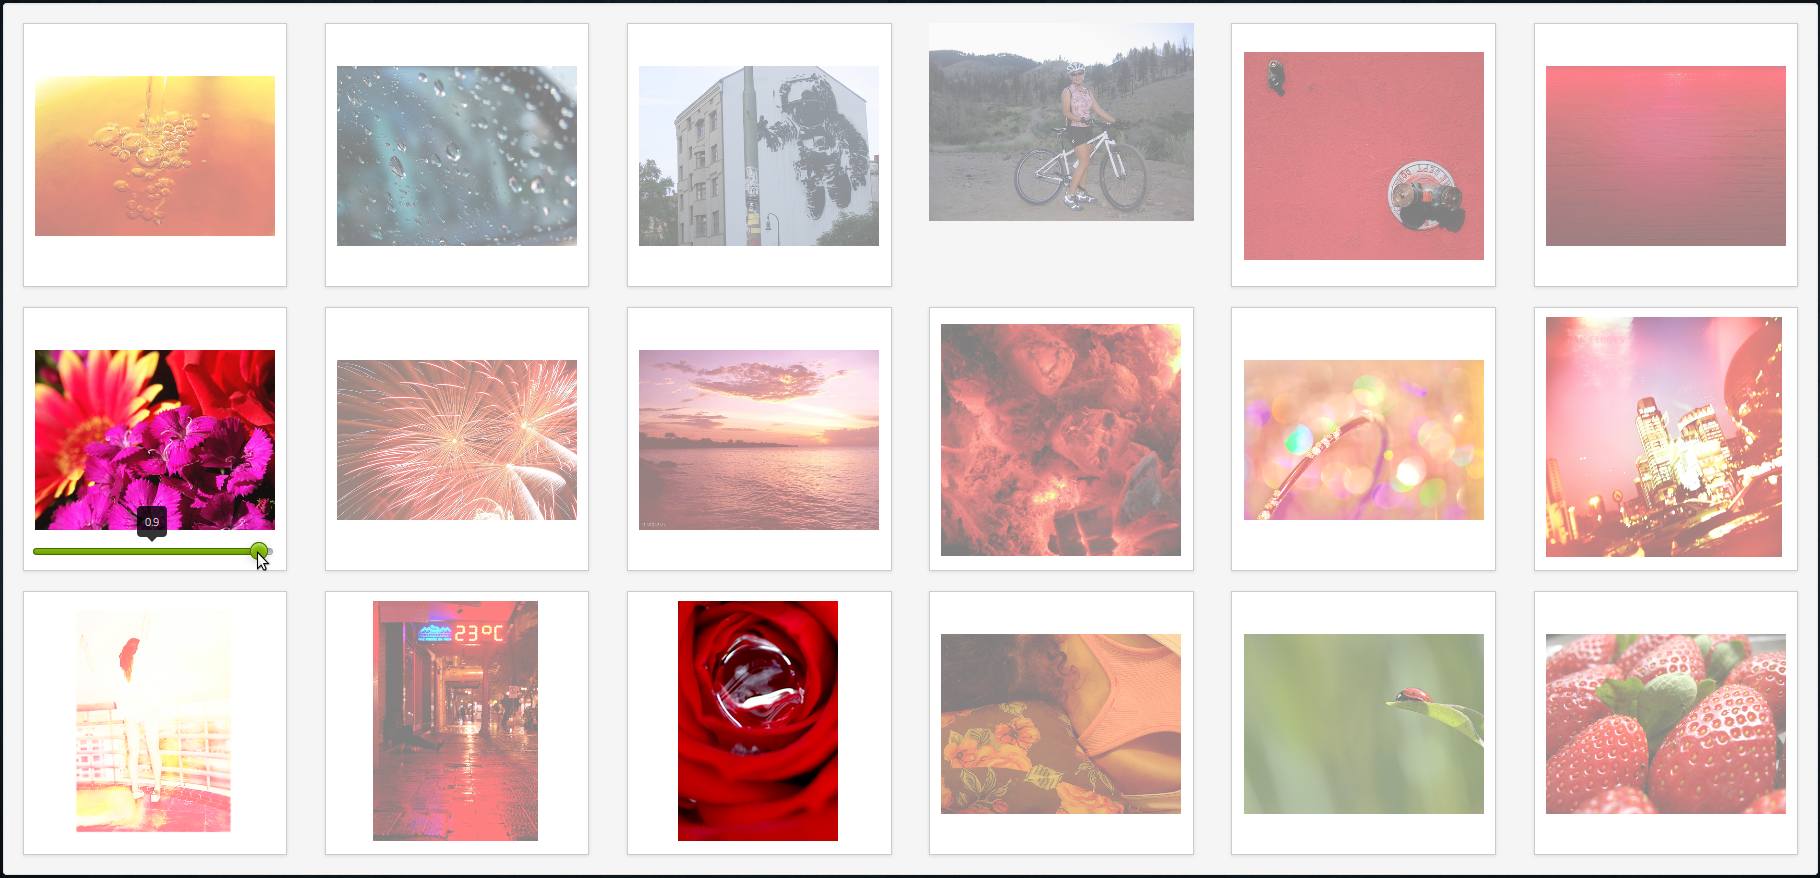
\includegraphics[width=0.90\textwidth,height=6cm]{figures/Rose_4.png}
    \caption{Red Rose Iteration 4}
    \label{red_rose_4}
\end{figure}

\begin{figure}[h!]
  \centering
    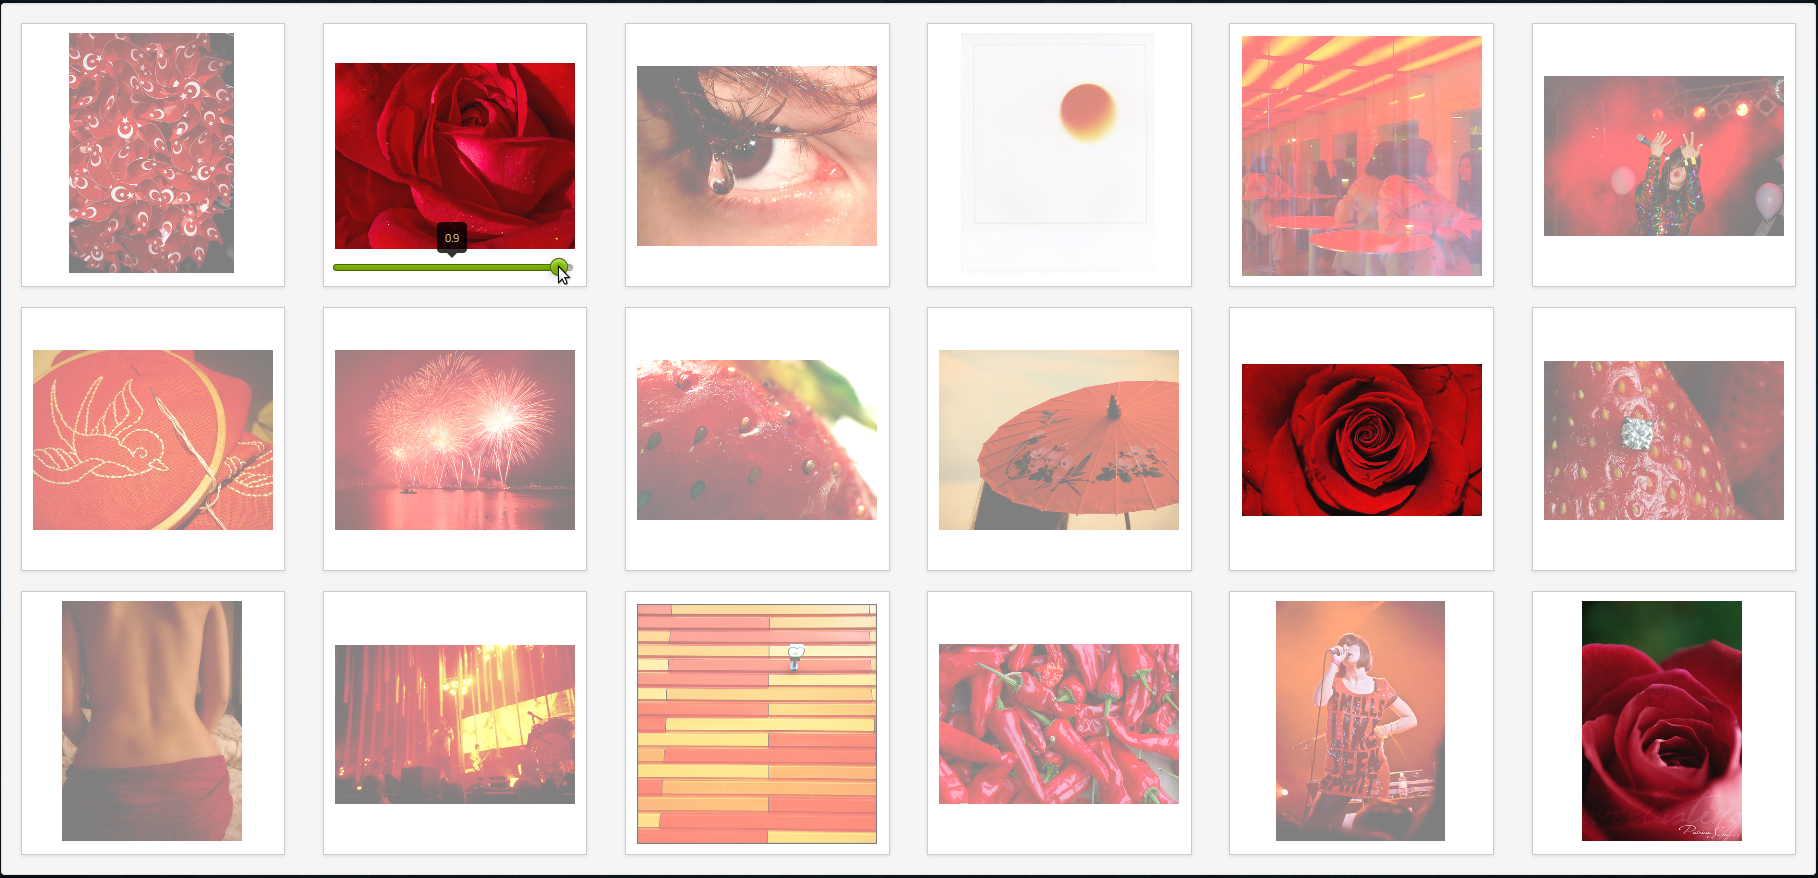
\includegraphics[width=0.90\textwidth,height=6cm]{figures/Rose_5.png}
    \caption{Red Rose Iteration 5}
    \label{red_rose_5}
\end{figure}


\begin{figure}[!h]
  \centering
    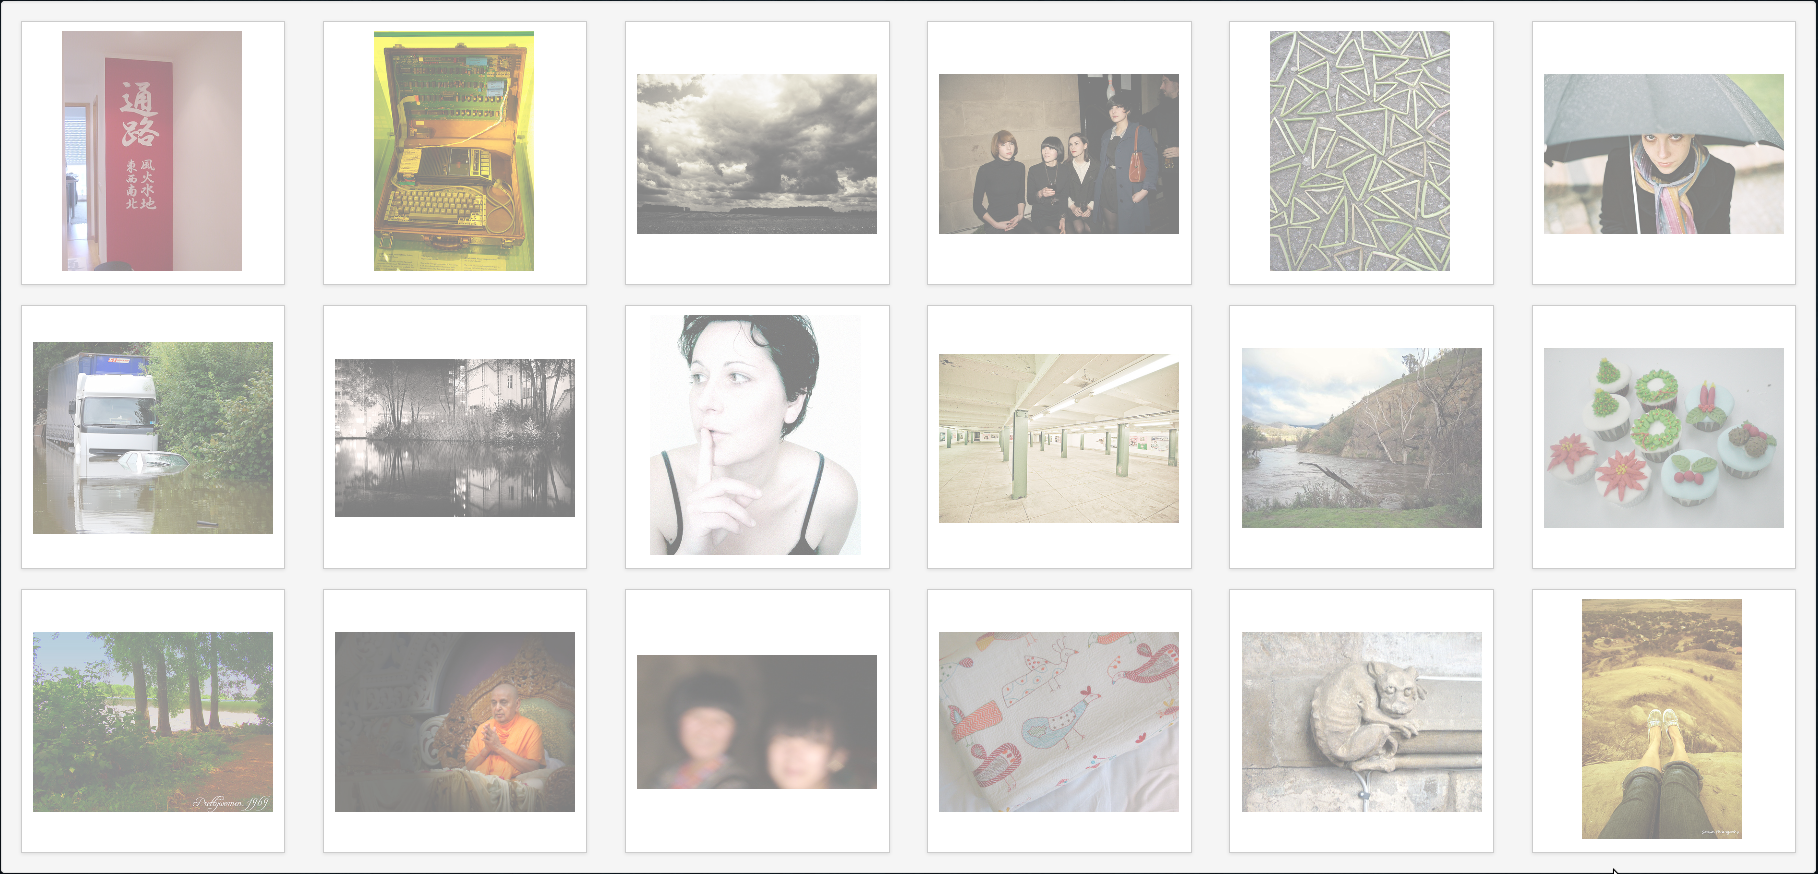
\includegraphics[width=0.90\textwidth,height=6cm]{figures/City_Night_1.png}
    \caption{City by night 1}
    \label{city_night_1}
\end{figure}

\begin{figure}[h!]
  \centering
    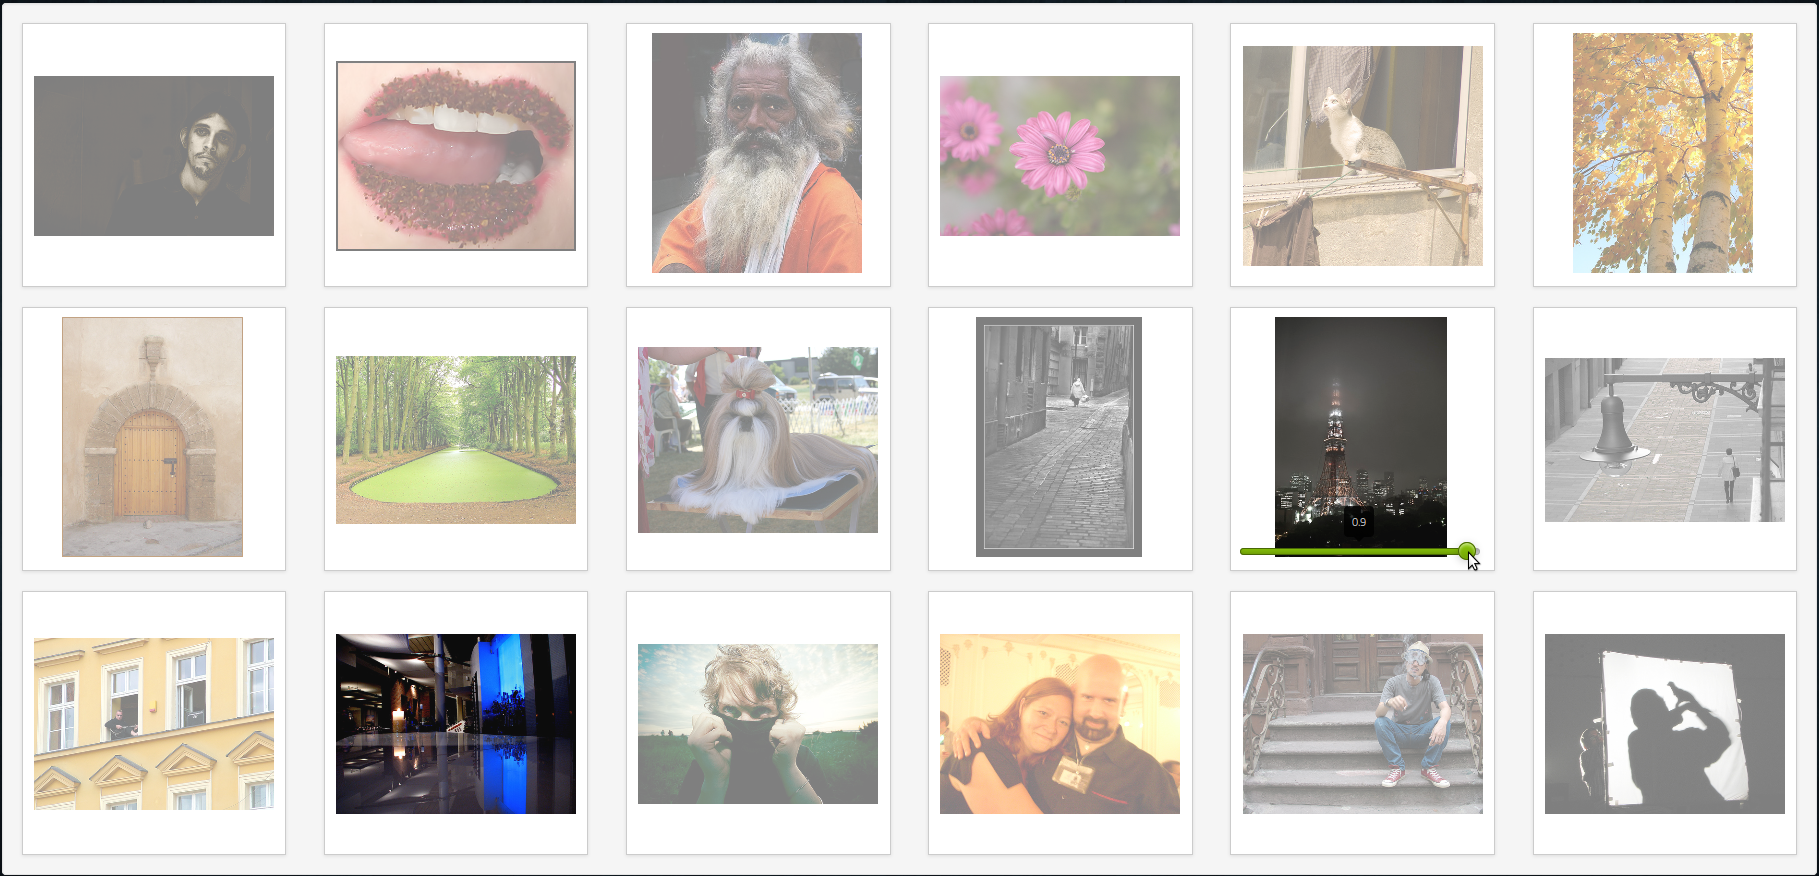
\includegraphics[width=0.90\textwidth,height=6cm]{figures/City_Night_2.png}
    \caption{City by night 2}
    \label{city_night_2}
\end{figure}

\begin{figure}[h!]
  \centering
    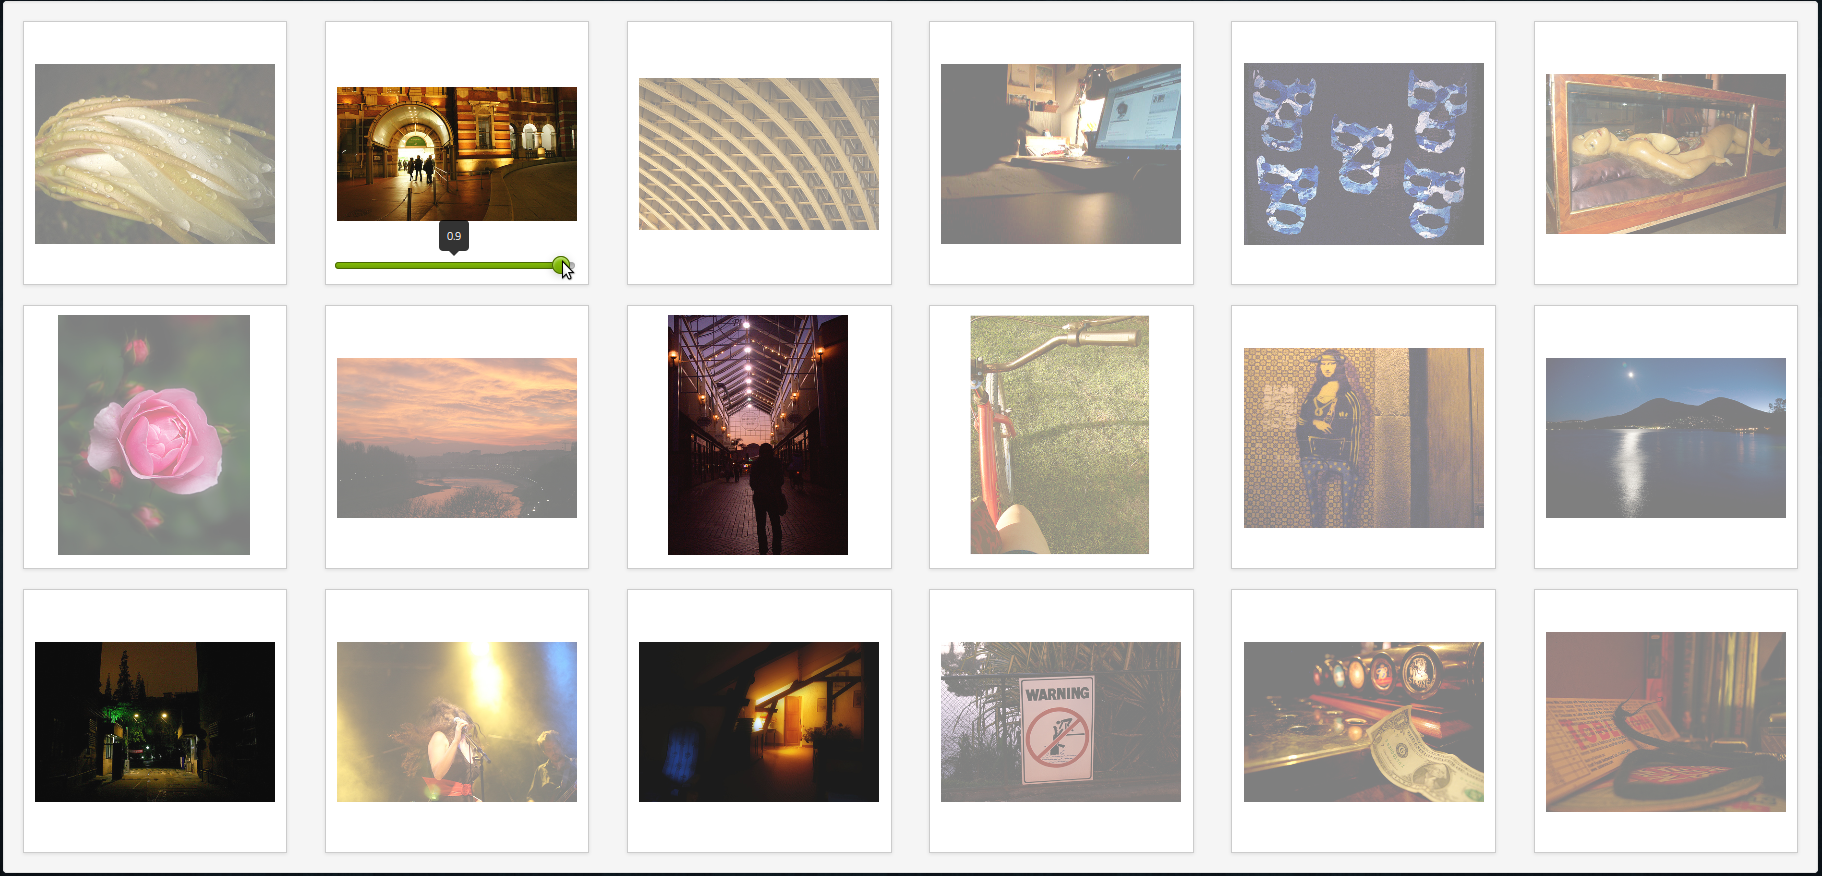
\includegraphics[width=0.90\textwidth,height=6cm]{figures/City_Night_3.png}
    \caption{City by night 3}
    \label{city_night_3}
\end{figure}

\begin{figure}[h!]
  \centering
    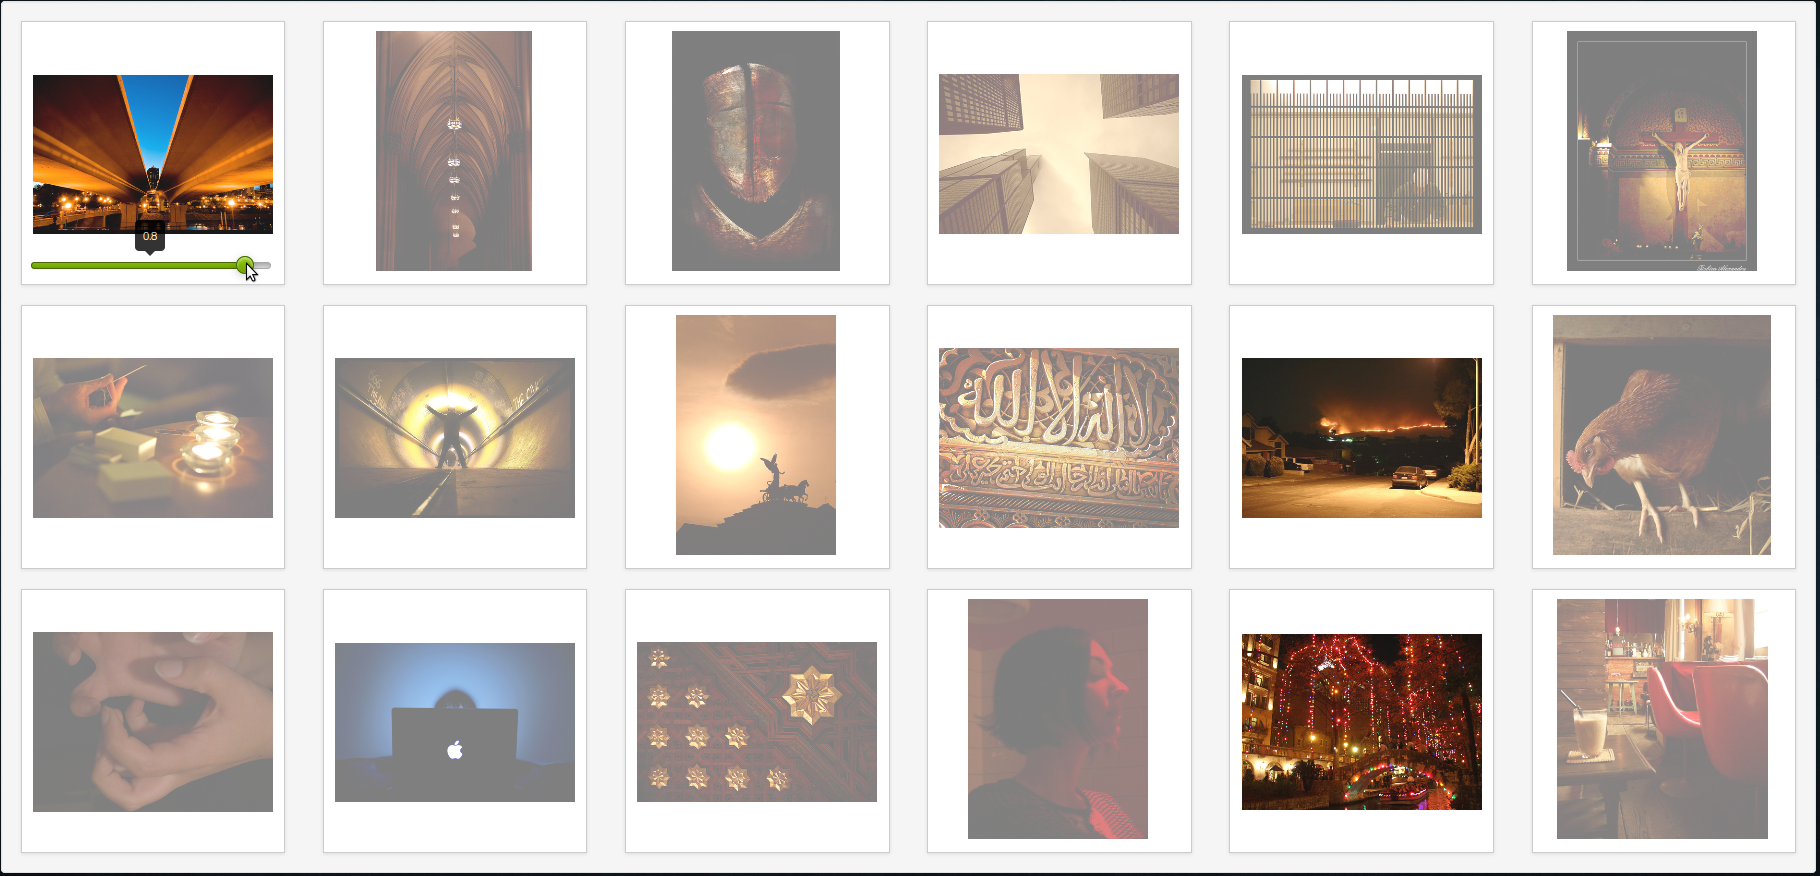
\includegraphics[width=0.90\textwidth,height=6cm]{figures/City_Night_4.png}
    \caption{City by night 4}
    \label{city_night_4}
\end{figure}

\begin{figure}[h!]
  \centering
    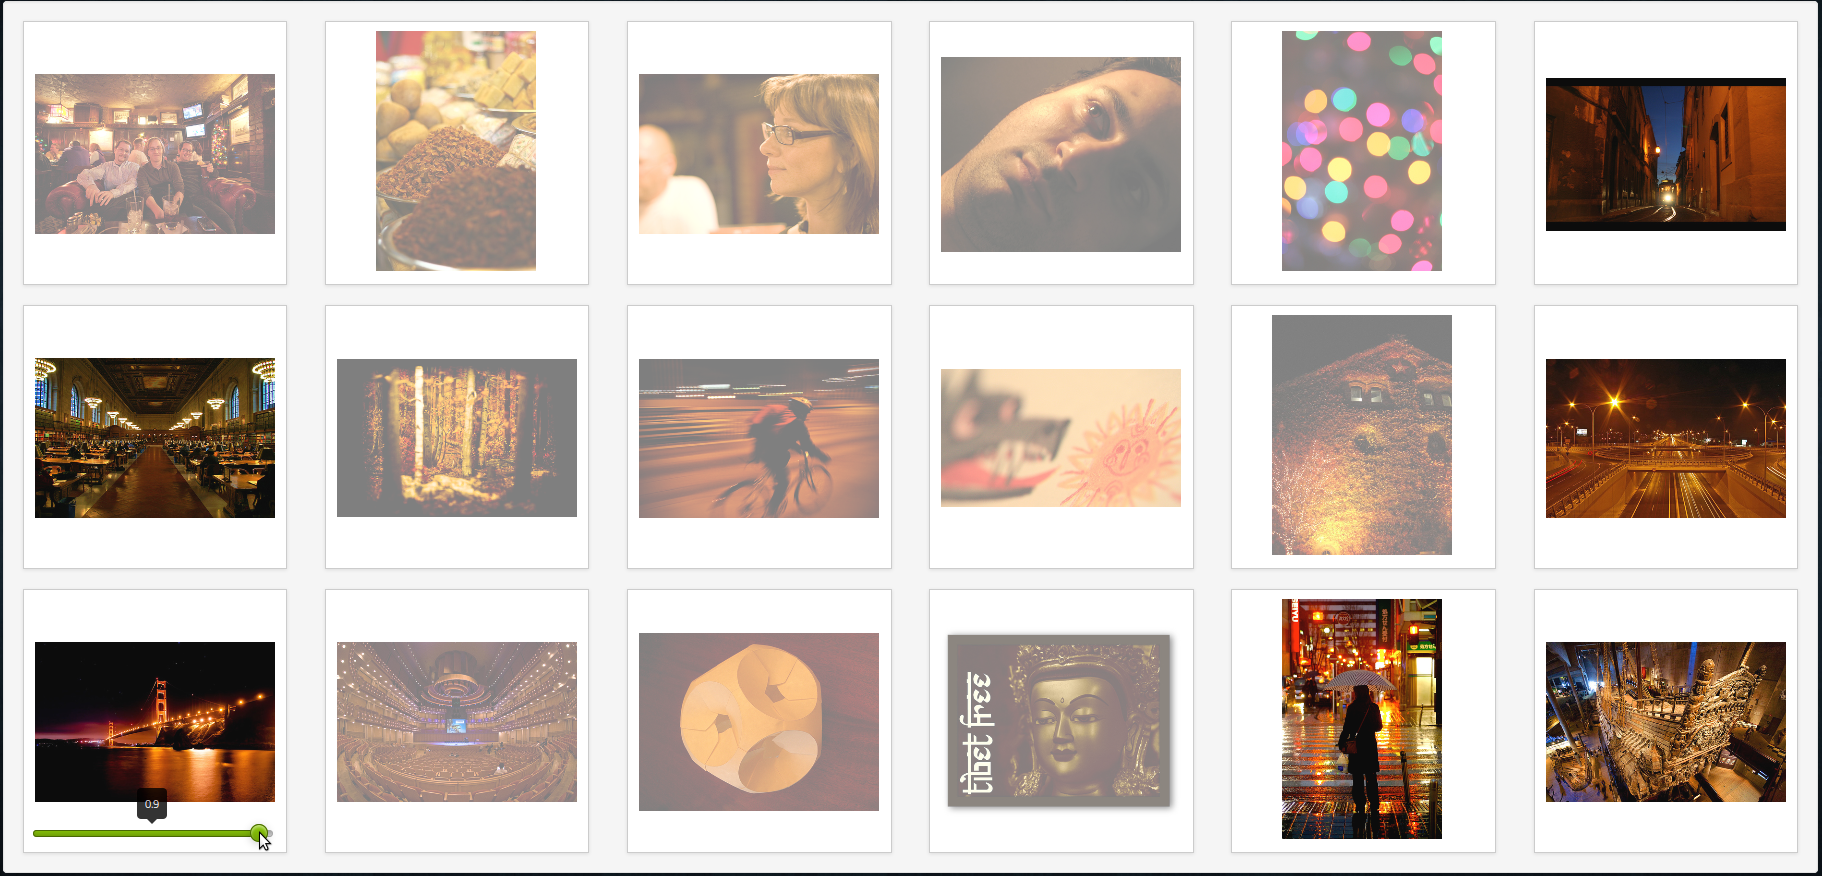
\includegraphics[width=0.90\textwidth,height=6cm]{figures/City_Night_5.png}
    \caption{City by night 5}
    \label{city_night_5}
\end{figure}


\section{Problems}

We have noticed issues from the results. One of the major issues is the applicability of GPUCB. It could not outperform EXPLOIT in target search. The reason is, once the user feedbacks a suitable image, say a "red rose", EXPLOIT will bring more red roses only. The probability that the user will like one of them the most and finish the search is highest in case of EXPLOIT. The exploration in GPUCB here might introduce some irrelevant images, thus prolonging the process of getting the most suitable "red rose". \\

On the contrary, sometimes it might be extremely useful to have exploration in target search. As we are showing random images initially, it might so happen that the user got no red, but a few reddish yellow images while starting. Assuming a reddish yellow to be the closest available match, the user gave a feedback to that. It is highly probable that EXPLOIT would bring up only reddish yellow images afterwards. Only exploration could bring up red images again to direct the search to a positive end. \\

As the first iteration shows images randomly, it might so happen that completely irrelevant images had been shown requiring the experiment to restart. \\

The system was slow in fetching images because gaussian process took a long time to run on CPU. \\

Once the user gives all the feedbacks he wants and moves to the next iteration, it might so happen that the outcome is not very favourable and the user might want to change some of the previous feedbacks. But it is not possible to go back and change the feedbacks. \\

We faced all these issues during the experiment. We have taken corrective measures for some of these and devised a second experiment which is discussed next.

\section{Experiment with FutureView}

In this experiment we introduce a new interface which helps eliminating the problem of users not being able to go back and change feedback if required. We split the screen into two sections, the left one having a width of 70\% and the right one 30\%. The left section has exactly the same structure of the display panel from the previous experiment but the right section is what we refer to as the FutureView. It also displays images but images here do not have any sliding-feedback controls and images appear a bit faded out. This view shows what images are going to appear in the next iteration if the user keeps the current feedbacks which is given to the images in the left section.

\begin{figure}[h!]
  \centering
    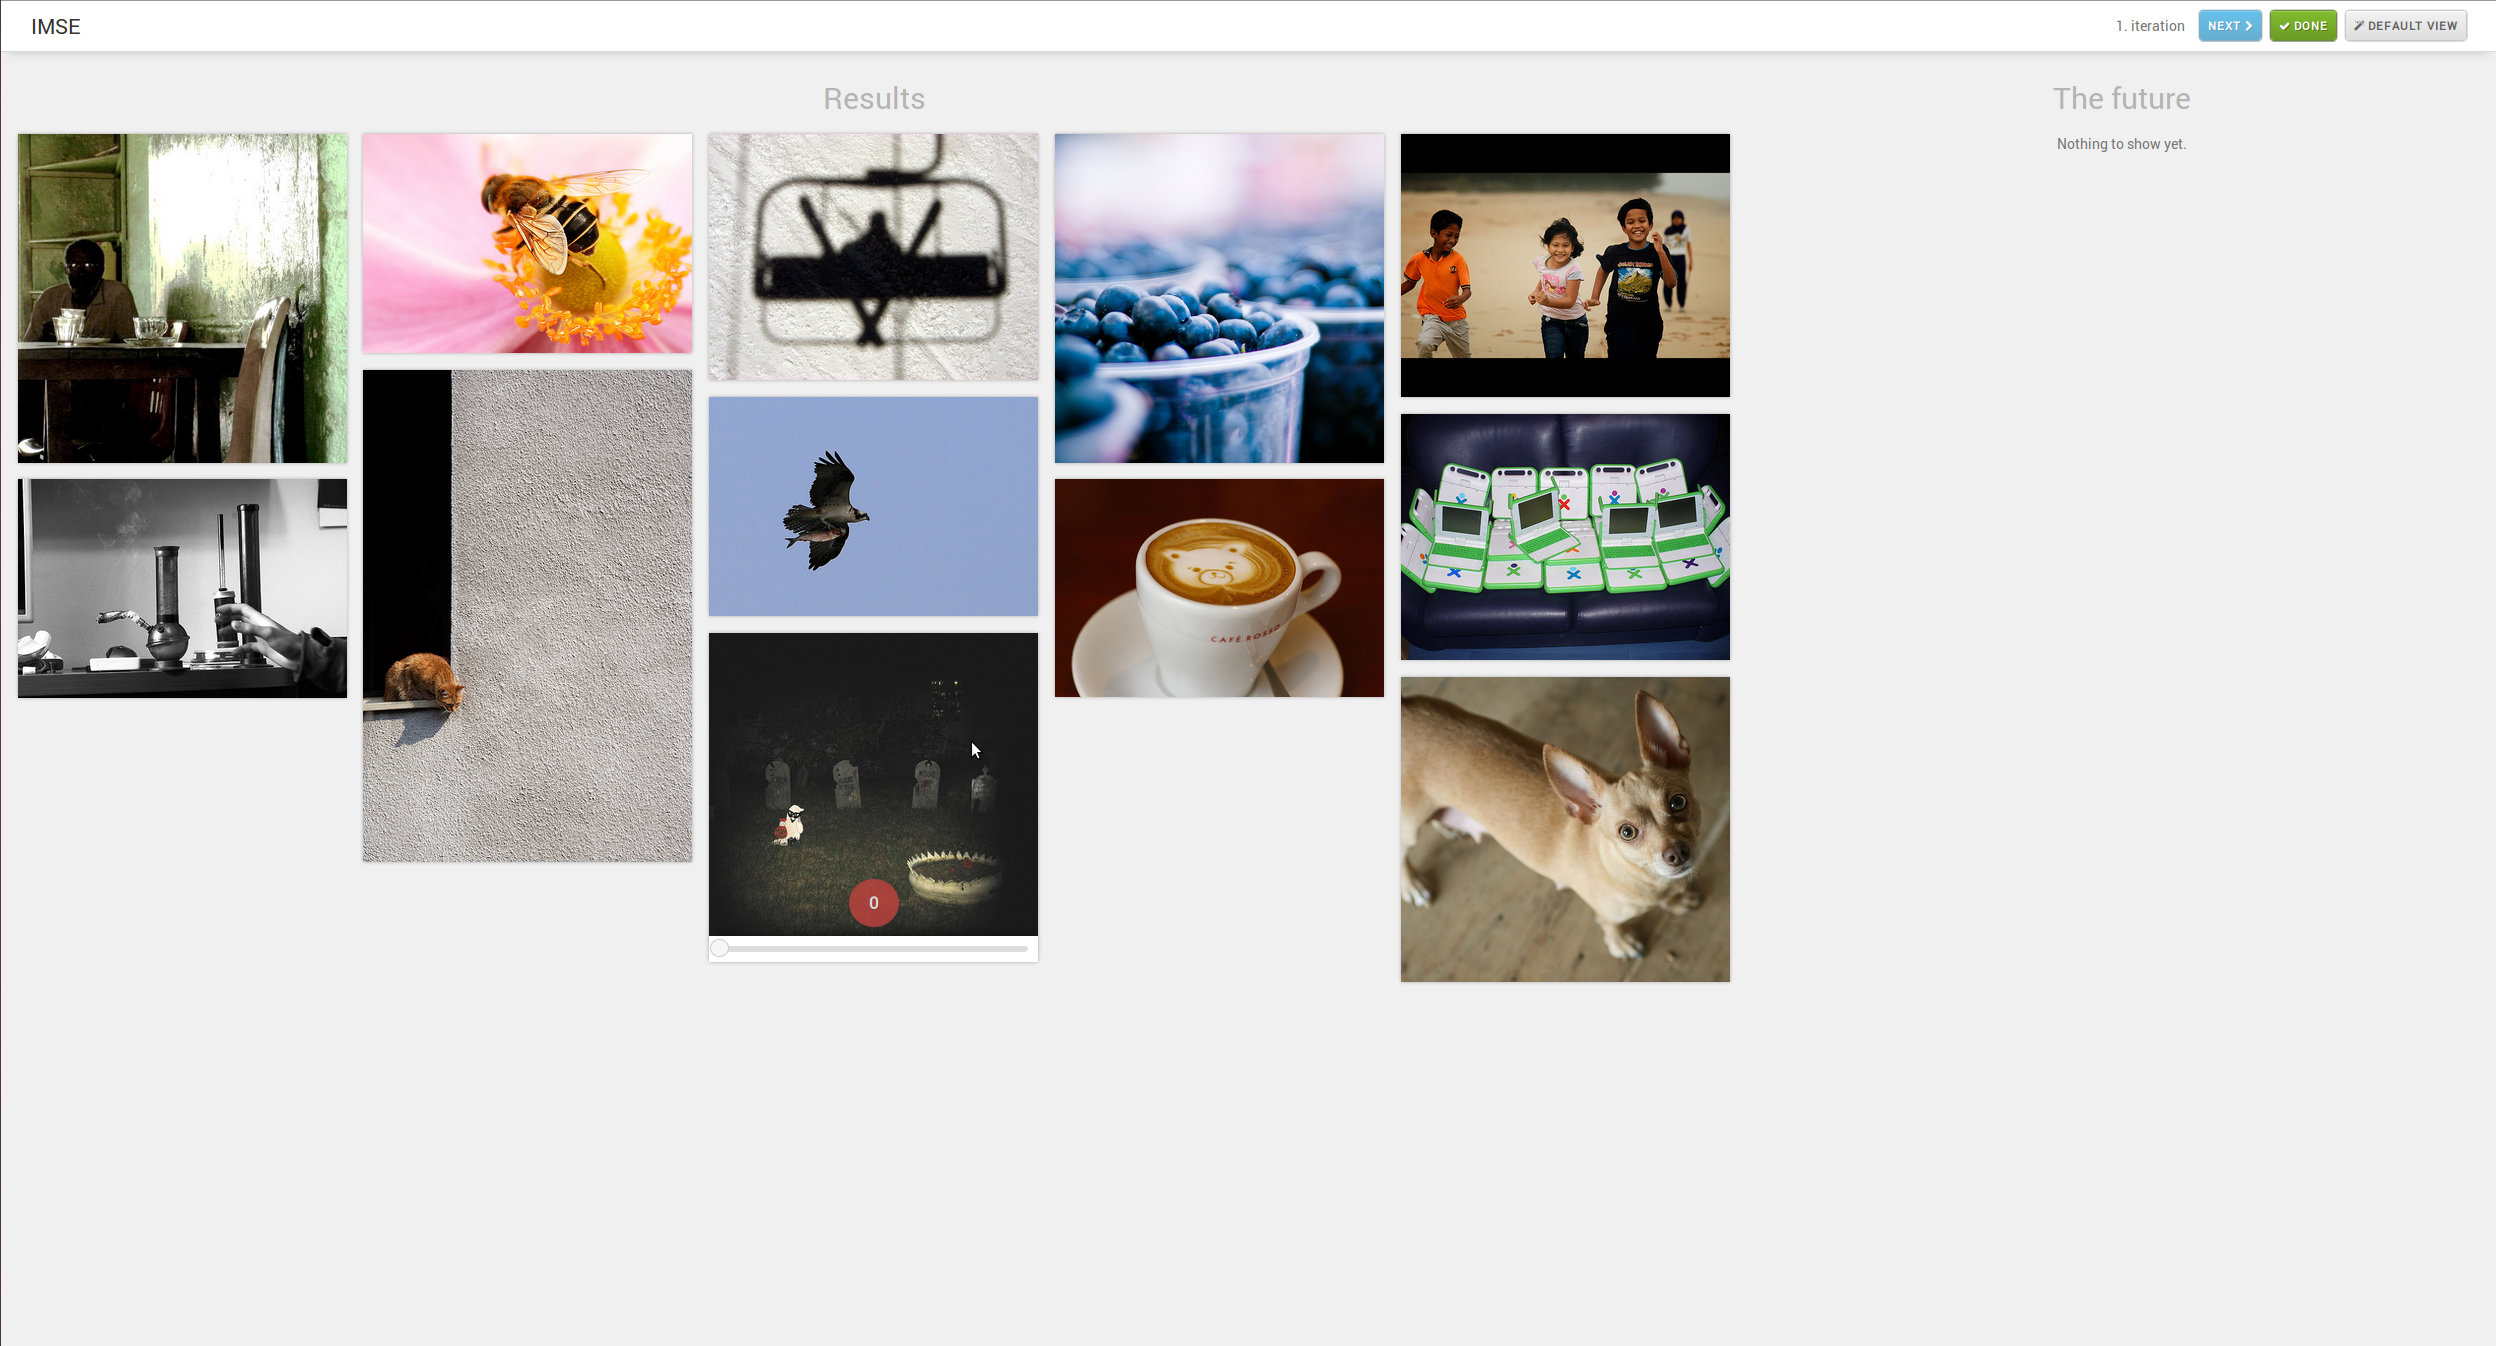
\includegraphics[width=0.90\textwidth,height=6cm]{figures/future_sample_1.jpg}
    \caption{Empty FutureView}
    \label{fut_samp_1}
\end{figure}

\begin{figure}[h!]
  \centering
    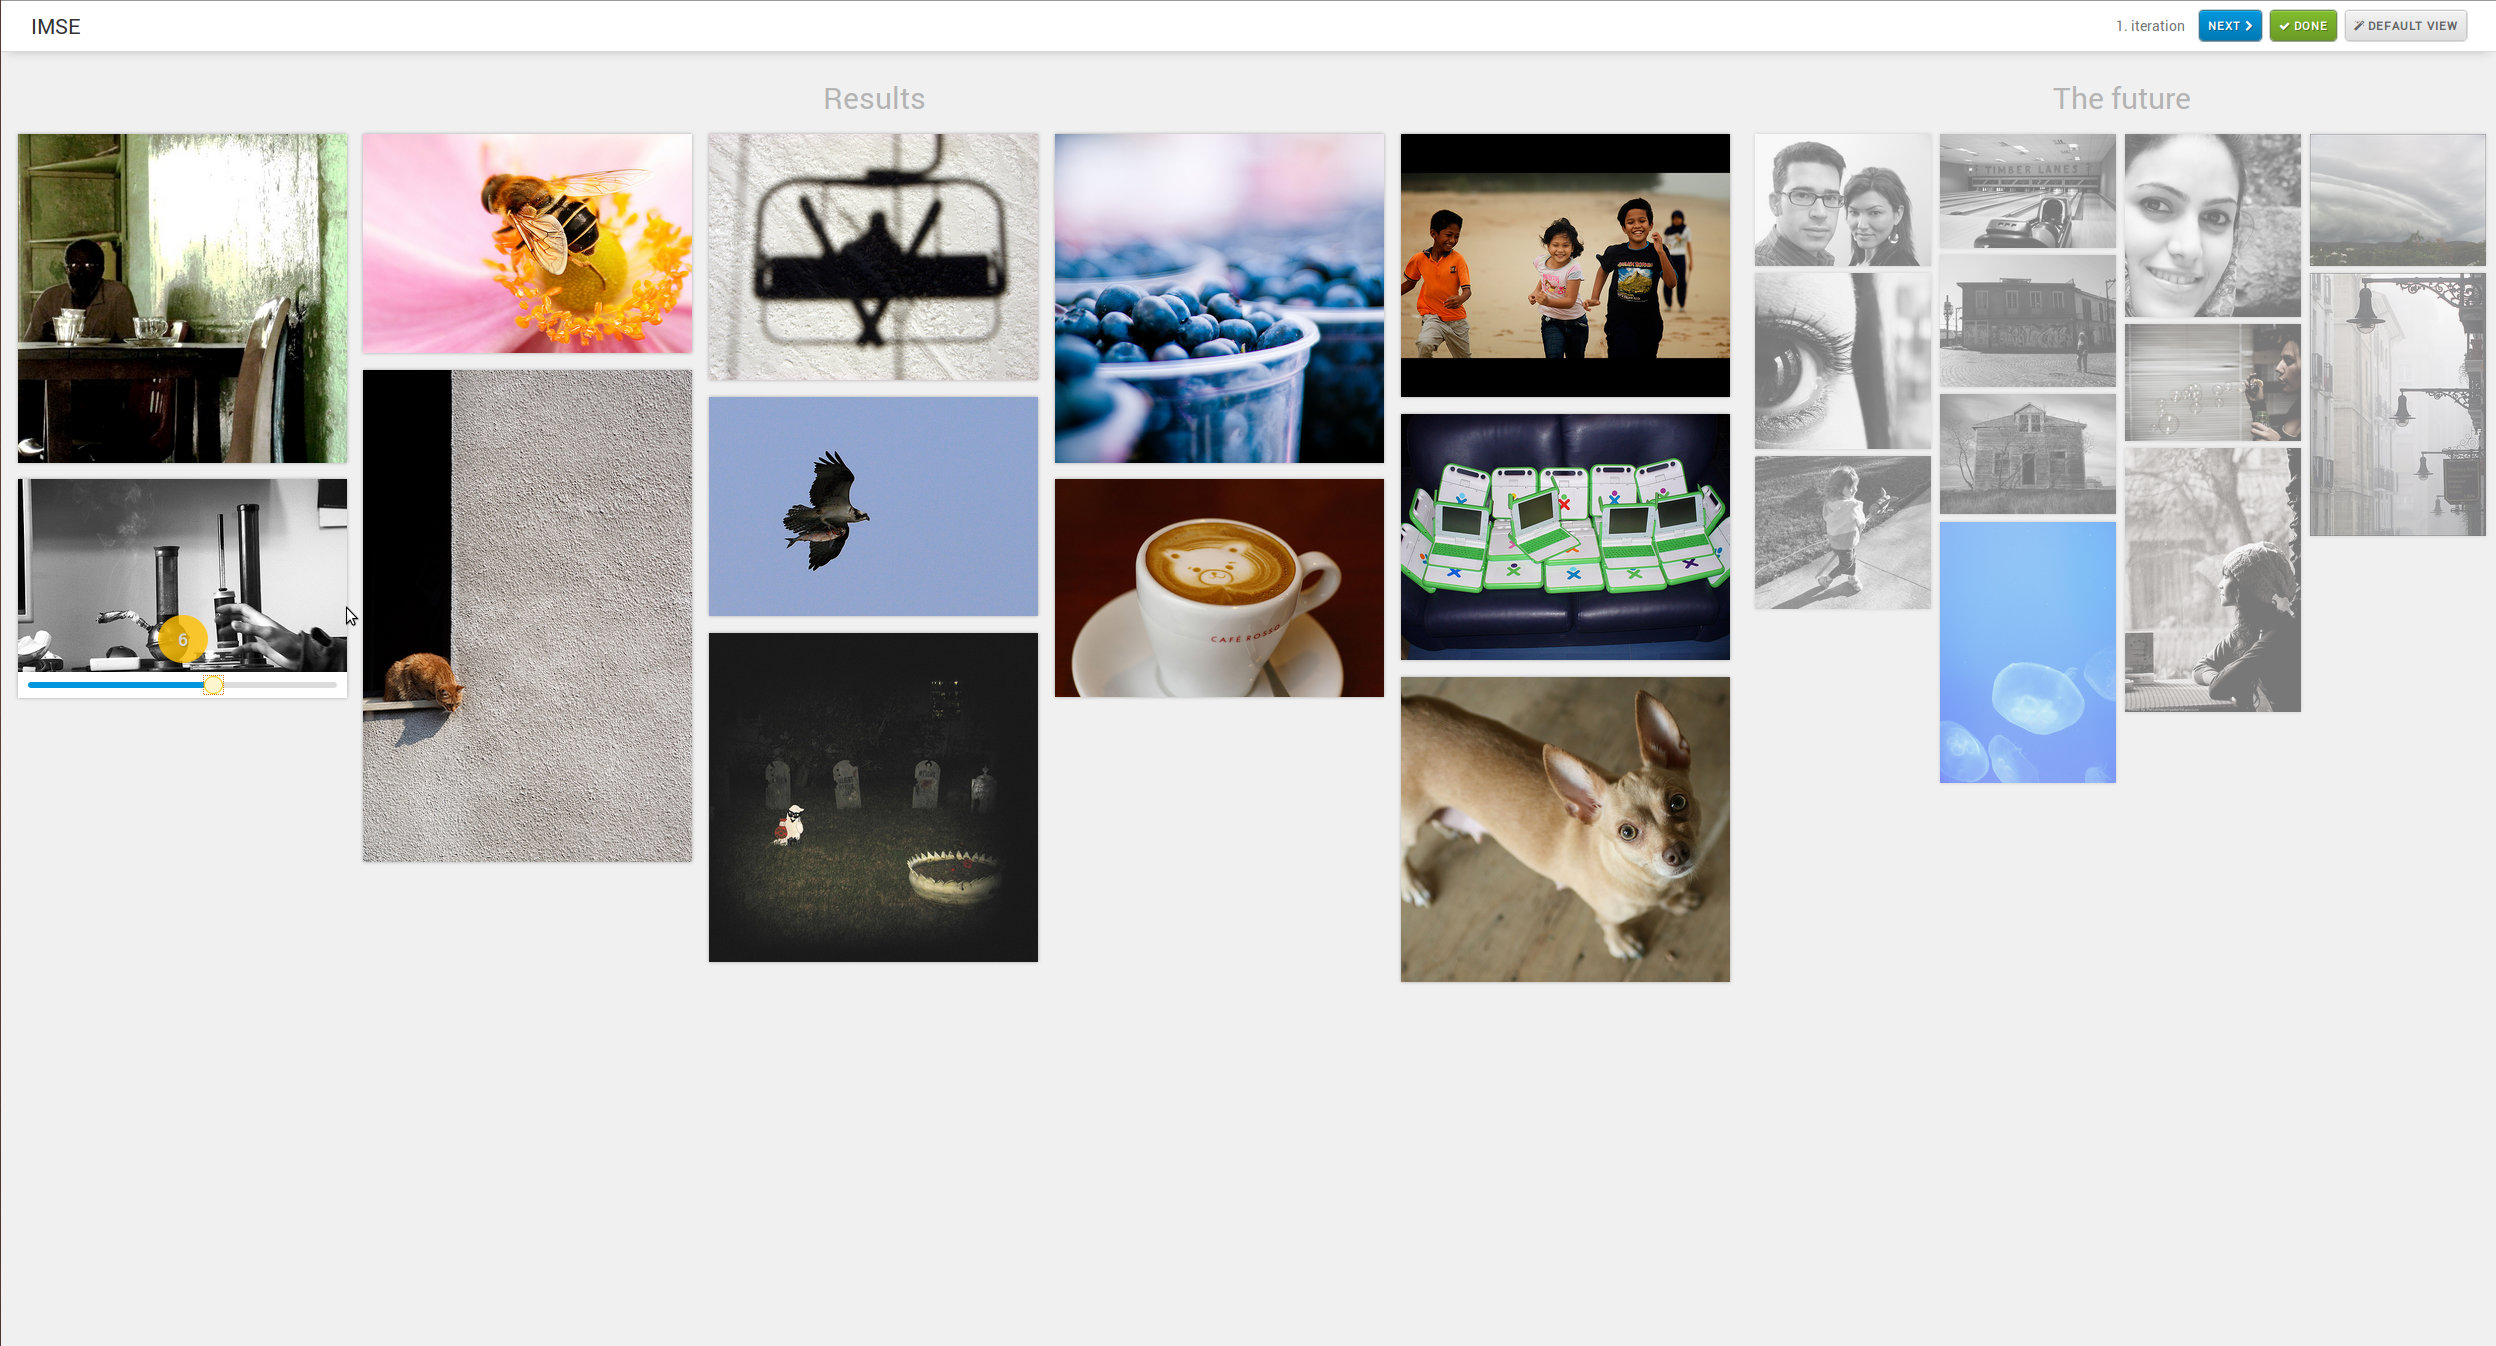
\includegraphics[width=0.90\textwidth,height=6cm]{figures/future_sample_2.jpg}
    \caption{FutureView filled up}
    \label{fut_samp_2}
\end{figure}

Therefore the user sees an early view of the next iteration. If images there are not suitable, the user can change the feedbacks and get new images. Once the user feels that the images in the FutureView are suitable, he can go next and the images from the FutureView will replace the images in the left section, we will refer to this as current view from now on, and the same procedure follows. Initially each iteration starts with an empty FutureView as shown in Figure: \ref{fut_samp_1} and as soon as the user gives one feedback, the FutureView fills up with images based on that feedback. Whenever the user gives a feedback to any of the images in the current view, the FutureView gets refreshed with new images as shown in Figure: \ref{fut_samp_2}.

\subsection{Participants}

We recruited 12 participants from the university with average age 24 (maximum 30, minimum 20). Three of these participants were females. Most of these participants were students, researchers and professionals in the field of computer science, one of them a mathematician.

\subsection{Tasks}

The tasks were divided into three broad genres, target search, category search and open ended search, as before. We had two tasks in each of these genre,

\begin{itemize}
	\item Target Search: Red Rose, Tall Building
	\item Category Search: City by Night, Seashore
	\item Open Ended Search: Happiness, Gardening
\end{itemize}

Our goal was to run a comparative study between the traditional view (current view) and FutureView over the same backend system to see which one performs better in terms of user satisfaction, task duration for an entire search session, amount of exploration over the image space etc.

We designed the experiments so that each participant had to perform 6 distinct tasks (Red Rose, Tall Building, City by Night, Seashore, Happiness and Gardening) altogether three being on the FutureView and the rest otherwise. We ensured each participant to perform only one task from a genre on each system (we refer to the current view and FutureView are two distinct systems), thus any participant who performed the task of red rose on current view, had to perform the task of tall building on FutureView as these two are from the same genre (target search). These scheme was followed for all three genres. This way we ensured that each participant performed three task (one from each genre) on single view and the rest, the other three task(left ones of each genre) on FutureView. This way we had $12 \times 3 = 36$ tasks performed on single view and $36$ tasks performed on FutureView. This also ensured that each task was performed $6$ times on each system.

In the previous experiment we had a random initial set to start with. But that led to having different impacts on the same task performed by different users. In this experiment, for each task, we kept a static initial set of images which can lead a user to the destination easily within $30$ iterations. The task allocation is shown in Table: \ref{table:table_task_allocation}. For each user and system combination, the three tasks were presented to the user one after another in random permutation.

We used a Tobii X2-60 eye tracker with sampling rate of 60Hz, to measure how much time a user spends to look at the FutureView, to analyse how a particular search is affected by the user's approach to the FutureView.

\begin{center}
    \begin{tabular}{ |l|l|l| }
		\hline
		\multicolumn{3}{ |c| }{Task distribution} \\
		\hline
		User serial number & Task performed on Single View & Task performed on FutureView \\ 
		\hline
		\multirow{3}{*}{1} & Red Rose & Tall Building \\
 			& City by Night & Seashore \\
 			& Happiness & Gardening \\
 		\hline
 		\multirow{3}{*}{2} & Red Rose & Tall Building \\
 			& Seashore & City by Night \\
 			& Gardening & Happiness \\
 		\hline
		\multirow{3}{*}{3} & Red Rose & Tall Building \\
 			& City by Night & Seashore \\
 			& Happiness & Gardening \\
 		\hline
 		\multirow{3}{*}{4} & Red Rose & Tall Building \\
 			& Seashore & City by Night \\
 			& Gardening & Happiness \\
 		\hline
 		\multirow{3}{*}{5} & Red Rose & Tall Building \\
 			& City by Night & Seashore \\
 			& Happiness & Gardening \\
 		\hline
 		\multirow{3}{*}{6} & Red Rose & Tall Building \\
 			& Seashore & City by Night \\
 			& Gardening & Happiness \\
 		\hline
 		\multirow{3}{*}{7} & Red Rose & Tall Building \\
 			& Seashore & City by Night \\
 			& Gardening & Happiness \\
 		\hline
 		\multirow{3}{*}{8} & Red Rose & Tall Building \\
 			& City by Night & Seashore \\
 			& Happiness & Gardening \\
 		\hline
 		\multirow{3}{*}{9} & Red Rose & Tall Building \\
 			& Seashore & City by Night \\
 			& Gardening & Happiness \\
 		\hline
 		\multirow{3}{*}{10} & Red Rose & Tall Building \\
 			& City by Night & Seashore \\
 			& Happiness & Gardening \\
 		\hline
 		\multirow{3}{*}{11} & Red Rose & Tall Building \\
 			& Seashore & City by Night \\
 			& Gardening & Happiness \\
 		\hline
 		\multirow{3}{*}{12} & Red Rose & Tall Building \\
 			& City by Night & Seashore \\
 			& Happiness & Gardening \\
 		\hline
	\end{tabular}
    \label{table:table_task_allocation}
\end{center}



\subsection{Procedure}


Each participant was given an instruction sheet to go through before the study along with a set of Warm Up questions in google form as follows,

\begin{itemize}
	\item How often do you search for images?
	\item How often do you search for images for work?
	\item How often do you search for images for leisure?
	\item What kind of images do you often search for?
	\item What are the image search systems you have used so far? Regular search engines or something more specific?
	\item What difficulties did you find in using traditional image search systems you have used?
	\item What changes you would be happy to see in your favourite image search engines?
\end{itemize}


After an user filled up the questionnaire and agreed upon the instructions, they were given a consent form to sign. The user was then introduced to both the systems and led through two training tasks on each of the systems. Once the user felt familiar, we calibrated the eye tracker and started logging user's gaze. Next we started the actual experiments. Six tasks were presented to the user in random order. After finishing each task, the user had to fill up a task usability questionnaire (modelled after NASA TLX questionnaire) and after every three tasks, i.e. after three experiments finished with each system, the user had to fill up a system usability questionnaire (modelled after SUS questionnaire). After all the six tasks finished, the eye tracker log is saved and we conducted a small interview with the user with mostly the following questions asked,

\begin{itemize}
	\item How was your experience with this system?
	\item How interesting was the system to use?
	\item Did you notice anything different, exciting, worth mentioning in this system that you did not see in other commercial image search systems you have used?
	\item Was the FutureView useful?
	\item Was the FutureView easy to use?
	\item Did the FutureView help you to reach your destination more quickly than the single view?
	\item What prospect do you see in this system if we make it a commercial one?
	\item Will you personally use this system regularly if we make it live on the internet?
	\item Do you feel any major functionality that an image search system should have and present in commercial systems, missing in our system?
	\item What suggestions for modifications, improvements do you have for this system?
\end{itemize}

\section{Results}

For each experiment we saved the number of iterations, running time, the images shown, the feedbacks received, the feedback timestamps and the end of experiment timestamps. Here we refer to each task as one experiment.

From these information we calculated the average iterations taken by experiments, average running time per iteration of experiments, average total running time of an entire experiment and average number of feedback received per experiment. Table\ref{table:exp_mean_genre} shows genre wise mean of all the parameters we calculated. Table \ref{table:exp_std_genre} shows the corresponding standard deviation. Table \ref{table:exp_wilcoxon_genre} shows the wilcoxon P value for each of the parameters comparing the FutureView and the single view. From Table \ref{table:exp_mean_genre} we see that the mean total running time is nearly equal in both the FutureView and single view but the average total images shown is much higher in FutureView than in single view across all the genres. We see from Table \ref{table:exp_wilcoxon_genre} that the P value is less than 0.05 in case of open and target searches and marginally over 0.05 in category search for total shown images and significantly greater than 0.05 for total duration. It supports the claim that total shown images is considerably higher in case of FutureView though it takes almost equal amount of time to finish. Therefore the FutureView allows much higher exploration in a lesser amount of time. Figure \ref{dur_vs_img} reflects the same.

\begin{figure}[h!]
  \centering
    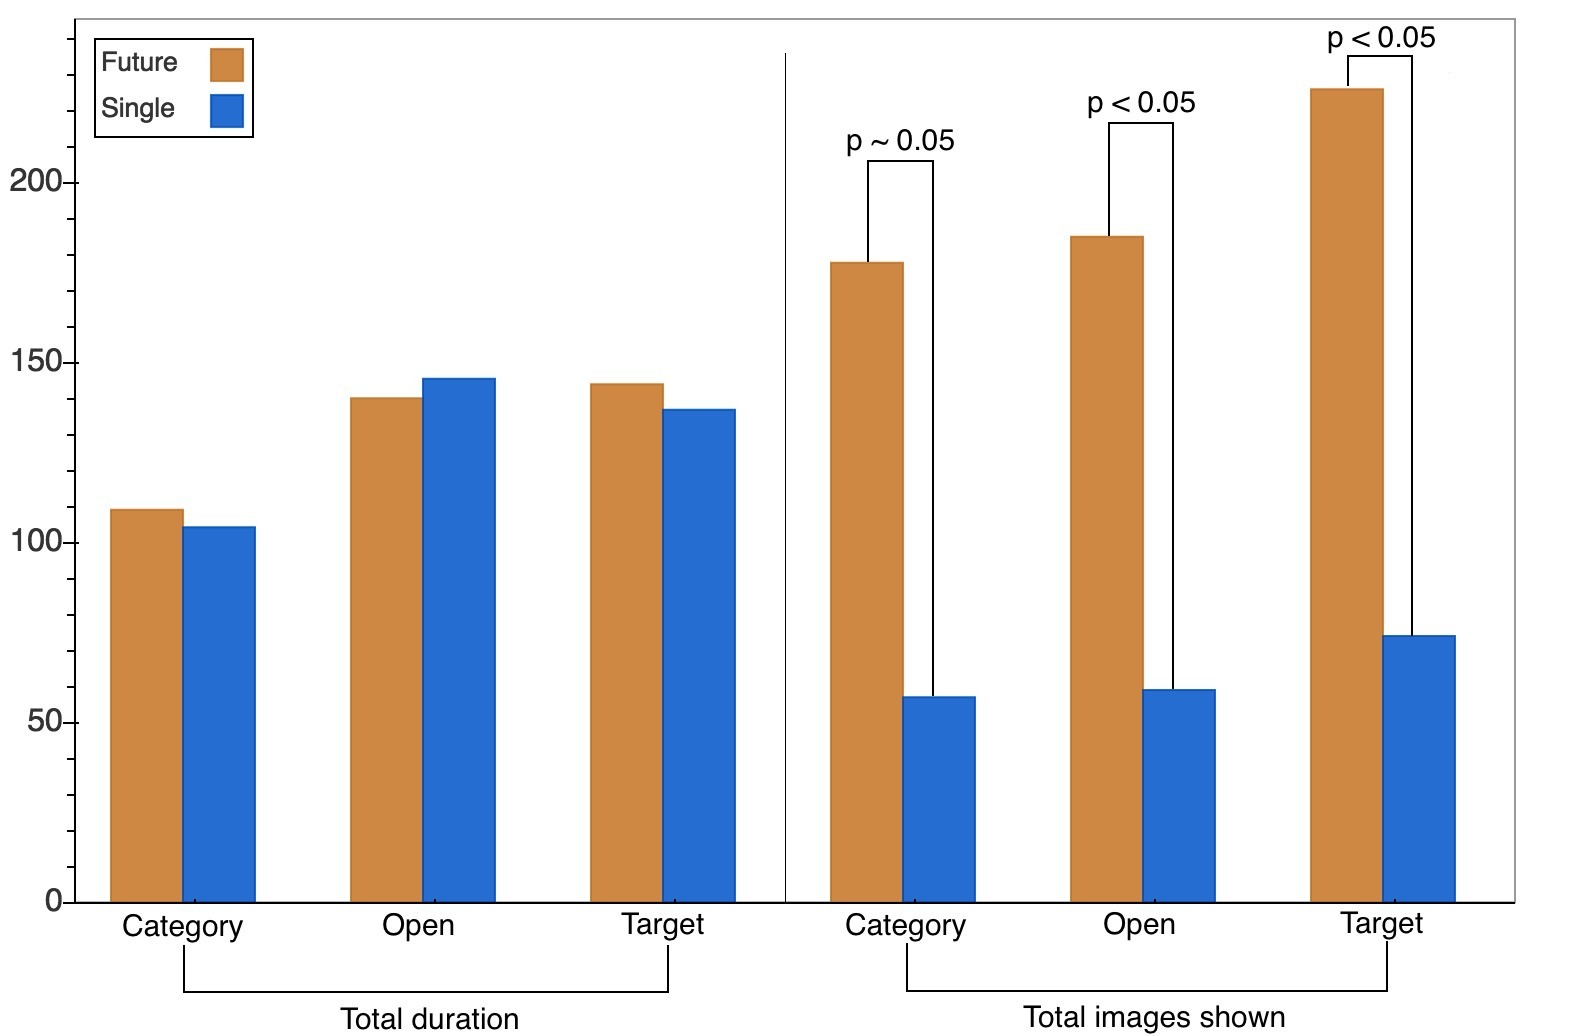
\includegraphics[width=0.95\textwidth,height=8cm]{figures/Bar_Chart__Duration_vs_Images.jpg}
    \caption{Total duration vs number of shown images}
    \label{dur_vs_img}
\end{figure}

\begin{table}
	\small
	\begin{center}
    \begin{tabular}{|l|r|r|r|r|r|r|}
        \hline
        \multicolumn{7}{|c|}{\textbf{Genre wise Mean}} \\
        \hline
        
        \multicolumn{1}{|c|}{} & \multicolumn{2}{|c|}{\textbf{Category}} & \multicolumn{2}{|c|}{\textbf{Open}} & \multicolumn{2}{|c|}{\textbf{Target}} \\
        \hline
        
        \multicolumn{1}{|c|}{} & \multicolumn{1}{|c|}{\textbf{Future}} & \multicolumn{1}{|c|}{\textbf{Single}} & \multicolumn{1}{|c|}{\textbf{Future}} & \multicolumn{1}{|c|}{\textbf{Single}} & \multicolumn{1}{|c|}{\textbf{Future}} & \multicolumn{1}{|c|}{\textbf{Single}} \\
        \hline
        
        \multicolumn{1}{|l|}{\textbf{Iterations}} & 14.83 & 4.75 & 15.42 & 4.92 & 18.83 & 6.17 \\
        \hline
        
        \multicolumn{1}{|l|}{\textbf{Avg. duration/Iteration (in Sec.)}} & 8.86 & 24.39 & 10.04 & 31.26 & 8.71 & 24.44 \\
        \hline
        
        \multicolumn{1}{|l|}{\textbf{Total duration (in Sec.)}} & 109.08 & 104.25 & 140.08 & 145.5 & 144 & 136.92 \\
        \hline
        
        \multicolumn{1}{|l|}{\textbf{Total shown images}} & 178 & 57 & 185 & 59 & 226 & 74 \\
        \hline
        
        \multicolumn{1}{|l|}{\textbf{Total feedback received}} & 14.83 & 9.33 & 15.42 & 17.5 & 18.83 & 15.58 \\
        \hline
        
    \end{tabular}
	\end{center}
	\caption{Genre wise Mean of experiment parameters}
    \label{table:exp_mean_genre}
\end{table}

% Genre wise standard deviation of experiment parameters

\begin{table}
	\small
	\begin{center}
    \begin{tabular}{|l|r|r|r|r|r|r|}
        \hline
        \multicolumn{7}{|c|}{\textbf{Genre wise Standard Deviation}} \\
        \hline
        
        \multicolumn{1}{|c|}{} & \multicolumn{2}{|c|}{\textbf{Category}} & \multicolumn{2}{|c|}{\textbf{Open}} & \multicolumn{2}{|c|}{\textbf{Target}} \\
        \hline
        
        \multicolumn{1}{|c|}{} & \multicolumn{1}{|c|}{\textbf{Future}} & \multicolumn{1}{|c|}{\textbf{Single}} & \multicolumn{1}{|c|}{\textbf{Future}} & \multicolumn{1}{|c|}{\textbf{Single}} & \multicolumn{1}{|c|}{\textbf{Future}} & \multicolumn{1}{|c|}{\textbf{Single}} \\
        \hline
        
        \multicolumn{1}{|l|}{\textbf{Iterations}} & 17.96 & 4.75 & 10.23 & 4.48 & 14.36 & 4.71 \\
        \hline
        
        \multicolumn{1}{|l|}{\textbf{Avg. duration/Iteration (in Sec.)}} & 2.96 & 4.41 & 4.06 & 10.83 & 2.8 & 11.55 \\
        \hline
        
        \multicolumn{1}{|l|}{\textbf{Total duration (in Sec.)}} & 101.72 & 101.11 & 84.13 & 123.42 & 95.11 & 105.33 \\
        \hline
        
        \multicolumn{1}{|l|}{\textbf{Total shown images}} & 215.57 & 57.01 & 122.75 & 53.78 & 172.37 & 56.48 \\
        \hline
        
        \multicolumn{1}{|l|}{\textbf{Total feedback received}} & 17.96 & 8.05 & 10.23 & 18.26 & 14.36 & 17.68 \\
        \hline
        
    \end{tabular}
	\end{center}
	\caption{Genre wise Standard Deviation of experiment parameters}
    \label{table:exp_std_genre}
\end{table}

% Genre wise Wilcoxon P value (FutureView vs Single View) of experiment parameters

\begin{table}
	\small
	\begin{center}
    \begin{tabular}{|l|r|r|r|}
        \hline
        \multicolumn{4}{|c|}{\textbf{Genre wise Wilcoxon P value}} \\
        \hline
        
        \multicolumn{1}{|c|}{} & \multicolumn{1}{|c|}{\textbf{Category}} & \multicolumn{1}{|c|}{\textbf{Open}} & \multicolumn{1}{|c|}{\textbf{Target}} \\
        \hline
        
        
        
        \multicolumn{1}{|l|}{\textbf{Iterations}} & 0.05405584757 & 0.003239921272 & 0.0206095954 \\
        \hline
        
        \multicolumn{1}{|l|}{\textbf{Avg. duration/Iteration (in Sec.)}} & 0.002217721464 & 0.002217721464 & 0.002217721464 \\
        \hline
        
        \multicolumn{1}{|l|}{\textbf{Total duration (in Sec.)}} & 0.8139453463 & 0.9687003809 & 0.6378701799 \\
        \hline
        
        \multicolumn{1}{|l|}{\textbf{Total shown images}} & 0.05405584757 & 0.003239921272 & 0.0206095954 \\
        \hline
        
        \multicolumn{1}{|l|}{\textbf{Total feedback received}} & 0.7891658874 & 0.7555407781 & 0.3461504513 \\
        \hline
        
    \end{tabular}
	\end{center}
	\caption{Genre wise Wilcoxon P value measure of experiment parameters (FutureView vs Single View)}
    \label{table:exp_wilcoxon_genre}
\end{table}

 In Table \ref{table:exp_mean_task}, \ref{table:exp_std_task} and \ref{table:exp_wilcox_task} show the task wise break up of the experiment parameters respectively. From Table \ref{table:exp_wilcox_task} we see that the total number of shown images is significantly higher in FutureView for city by night, gardening, happiness and tall building. Though for red rose and seashore it did not pass the threshold of statistical significance (p < 0.05), from Table \ref{table:exp_mean_task} we see that the mean total shown images is much higher in FutureView for those two tasks thus resulting a cumulative higher number overall for each genre.

% Task wise mean of experiment parameters

\begin{table}
	\small
	\begin{center}
    \begin{tabular}{|l|r|r|r|r|r|r|}
        \hline
        \multicolumn{7}{|c|}{\textbf{Task wise Mean}} \\
        \hline
        
        \multicolumn{1}{|c|}{} & \multicolumn{2}{|c|}{\textbf{City by Night}} & \multicolumn{2}{|c|}{\textbf{Gardening}} & \multicolumn{2}{|c|}{\textbf{Happiness}} \\
        \hline
        
        \multicolumn{1}{|c|}{} & \multicolumn{1}{|c|}{\textbf{Future}} & \multicolumn{1}{|c|}{\textbf{Single}} & \multicolumn{1}{|c|}{\textbf{Future}} & \multicolumn{1}{|c|}{\textbf{Single}} & \multicolumn{1}{|c|}{\textbf{Future}} & \multicolumn{1}{|c|}{\textbf{Single}} \\
        \hline
        
        \multicolumn{1}{|l|}{\textbf{Iterations}} & 8.33 & 2.5 & 16.33 & 7 & 14.50 & 2.83 \\
        \hline
        
        \multicolumn{1}{|l|}{\textbf{Avg. duration/Iteration (in Sec.)}} & 9.87 & 24.7 & 8.83 & 31.24 & 11.25 & 31.27 \\
        \hline
        
        \multicolumn{1}{|l|}{\textbf{Total duration (in Sec.)}} & 82.83 & 54.17 & 136.83 & 209 & 143.33 & 82 \\
        \hline
        
        \multicolumn{1}{|l|}{\textbf{Total shown images}} & 100 & 30 & 196 & 84 & 174 & 34 \\
        \hline
        
        \multicolumn{1}{|l|}{\textbf{Total feedback received}} & 8.33 & 4.67 & 16.33 & 25.5 & 14.5 & 9.5 \\
        \hline
        \hline
        \multicolumn{1}{|c|}{} & \multicolumn{2}{|c|}{\textbf{Red Rose}} & \multicolumn{2}{|c|}{\textbf{Seashore}} & \multicolumn{2}{|c|}{\textbf{Tall Building}} \\
        \hline
        
        \multicolumn{1}{|c|}{} & \multicolumn{1}{|c|}{\textbf{Future}} & \multicolumn{1}{|c|}{\textbf{Single}} & \multicolumn{1}{|c|}{\textbf{Future}} & \multicolumn{1}{|c|}{\textbf{Single}} & \multicolumn{1}{|c|}{\textbf{Future}} & \multicolumn{1}{|c|}{\textbf{Single}} \\
        \hline
        
        \multicolumn{1}{|l|}{\textbf{Iterations}} & 23.83 & 7.67 & 21.33 & 7 & 13.83 & 4.67 \\
        \hline
        
        \multicolumn{1}{|l|}{\textbf{Avg. duration/Iteration (in Sec.)}} & 9.04 & 20.58 & 7.84 & 24.09 & 8.37 & 28.3 \\
        \hline
        
        \multicolumn{1}{|l|}{\textbf{Total duration (in Sec.)}} & 169.5 & 157 & 135.33 & 154.33 & 118.5 & 116.83 \\
        \hline
        
        \multicolumn{1}{|l|}{\textbf{Total shown images}} & 286 & 92 & 256 & 84 & 166 & 56 \\
        \hline
        
        \multicolumn{1}{|l|}{\textbf{Total feedback received}} & 23.83 & 22.33 & 21.33 & 14 & 13.83 & 8.83 \\
        \hline

    \end{tabular}
	\end{center}
	\caption{Task wise Mean of experiment parameters}
    \label{table:exp_mean_task}
\end{table}



% Task wise standard deviation of experiment parameters

\begin{table}
	\small
	\begin{center}
    \begin{tabular}{|l|r|r|r|r|r|r|}
        \hline
        \multicolumn{7}{|c|}{\textbf{Task wise Standard Deviation}} \\
        \hline
        
        \multicolumn{1}{|c|}{} & \multicolumn{2}{|c|}{\textbf{City by Night}} & \multicolumn{2}{|c|}{\textbf{Gardening}} & \multicolumn{2}{|c|}{\textbf{Happiness}} \\
        \hline
        
        \multicolumn{1}{|c|}{} & \multicolumn{1}{|c|}{\textbf{Future}} & \multicolumn{1}{|c|}{\textbf{Single}} & \multicolumn{1}{|c|}{\textbf{Future}} & \multicolumn{1}{|c|}{\textbf{Single}} & \multicolumn{1}{|c|}{\textbf{Future}} & \multicolumn{1}{|c|}{\textbf{Single}} \\
        \hline
        
        \multicolumn{1}{|l|}{\textbf{Iterations}} & 5.05 & 2.35 & 8.45 & 5.76 & 12.52 & 0.75 \\
        \hline
        
        \multicolumn{1}{|l|}{\textbf{Avg. duration/Iteration (in Sec.)}} & 3.5 & 5.02 & 2.58 & 11.17 & 5.1 & 11.55 \\
        \hline
        
        \multicolumn{1}{|l|}{\textbf{Total duration (in Sec.)}} & 58.99 & 42.75 & 74.83 & 153.56 & 99.73 & 15.89 \\
        \hline
        
        \multicolumn{1}{|l|}{\textbf{Total shown images}} & 60.56 & 28.14 & 101.45 & 69.14 & 150.22 & 9.03 \\
        \hline
        
        \multicolumn{1}{|l|}{\textbf{Total feedback received}} & 5.05 & 3.56 & 8.45 & 23.97 & 12.52 & 2.35 \\
        \hline
        \hline
        \multicolumn{1}{|c|}{} & \multicolumn{2}{|c|}{\textbf{Red Rose}} & \multicolumn{2}{|c|}{\textbf{Seashore}} & \multicolumn{2}{|c|}{\textbf{Tall Building}} \\
        \hline
        
        \multicolumn{1}{|c|}{} & \multicolumn{1}{|c|}{\textbf{Future}} & \multicolumn{1}{|c|}{\textbf{Single}} & \multicolumn{1}{|c|}{\textbf{Future}} & \multicolumn{1}{|c|}{\textbf{Single}} & \multicolumn{1}{|c|}{\textbf{Future}} & \multicolumn{1}{|c|}{\textbf{Single}} \\
        \hline
        
        \multicolumn{1}{|l|}{\textbf{Iterations}} & 18.17 & 6.09 & 24.15 & 5.66 & 7.99 & 2.5 \\
        \hline
        
        \multicolumn{1}{|l|}{\textbf{Avg. duration/Iteration (in Sec.)}} & 3.67 & 2.8 & 2.13 & 4.18 & 1.87 & 15.81 \\
        \hline
        
        \multicolumn{1}{|l|}{\textbf{Total duration (in Sec.)}} & 112.02 & 137.22 & 132.78 & 121.01 & 76.11 & 67.91 \\
        \hline
        
        \multicolumn{1}{|l|}{\textbf{Total shown images}} & 218.05 & 73.06 & 289.76 & 67.88 & 95.82 & 30.04 \\
        \hline
        
        \multicolumn{1}{|l|}{\textbf{Total feedback received}} & 18.17 & 23.37 & 24.15 & 8.81 & 7.99 & 5.67 \\
        \hline

    \end{tabular}
	\end{center}
	\caption{Task wise Standard Deviation of experiment parameters}
    \label{table:exp_std_task}
\end{table}

% Task wise Wilcoxon P value (FutureView vs Single View) of experiment parameters

\begin{table}
	\small
	\begin{center}
    \begin{tabular}{|l|r|r|r|}
        \hline
        \multicolumn{4}{|c|}{\textbf{Task wise Wilcoxon P value}} \\
        \hline
        
        
        
        \multicolumn{1}{|c|}{} & \multicolumn{1}{|c|}{\textbf{City by Night}} & \multicolumn{1}{|c|}{\textbf{Gardening}} & \multicolumn{1}{|c|}{\textbf{Happiness}} \\
        \hline
        
        \multicolumn{1}{|l|}{\textbf{Iterations}} & 0.07473549831 & 0.02770784936 & 0.02770784936 \\
        \hline
        
        \multicolumn{1}{|l|}{\textbf{Avg. duration/Iteration (in Sec.)}} & 0.02770784936 & 0.02770784936 & 0.04639946187 \\
        \hline
        
        \multicolumn{1}{|l|}{\textbf{Total duration (in Sec.)}} & 0.3454475305 & 0.3454475305 & 0.172954918 \\
        \hline
        
        \multicolumn{1}{|l|}{\textbf{Total shown images}} & 0.07473549831 & 0.02770784936 & 0.02770784936 \\
        \hline
        
        \multicolumn{1}{|l|}{\textbf{Total feedback received}} & 0.2071604489 & 0.3454475305 & 0.5282327769 \\
        \hline
        \hline
        
        \multicolumn{1}{|c|}{} & \multicolumn{1}{|c|}{\textbf{Red Rose}} & \multicolumn{1}{|c|}{\textbf{Seashore}} & \multicolumn{1}{|c|}{\textbf{Tall Building}} \\
        \hline
		
		\multicolumn{1}{|l|}{\textbf{Iterations}} & 0.172954918 & 0.1380107376 & 0.02728117148 \\
        \hline
        
        \multicolumn{1}{|l|}{\textbf{Avg. duration/Iteration (in Sec.)}} & 0.02770784936 & 0.02770784936 & 0.02770784936 \\
        \hline
        
        \multicolumn{1}{|l|}{\textbf{Total duration (in Sec.)}} & 0.6001794871 & 0.6001794871 & 0.9165119079 \\
        \hline
        
        \multicolumn{1}{|l|}{\textbf{Total shown images}} & 0.172954918 & 0.1380107376 & 0.02728117148 \\
        \hline
        
        \multicolumn{1}{|l|}{\textbf{Total feedback received}} & 0.5001842571 & 0.752493649 & 0.1380107376 \\
        \hline
        
    \end{tabular}
	\end{center}
	\caption{Task wise Wilcoxon P value measure of experiment parameters (FutureView vs Single View)}
    \label{table:exp_wilcox_task}
\end{table}

We also calculated the aggregates on usability parameters extracted from the NASA  TLX questionnaire the users had to fill up after every task ended. These parameters were rated in a scale from 1 to 10. From Table \ref{table:use_mean_genre} we see that for all the genres, the users felt more successful in the FutureView. It also shows that the amount of hard work needed in accomplishing the tasks were more in single view in category search and target search. For open ended search it went otherwise. The reason could be that as the nature of the task did not give any fixed target, the users were diverted a bit when they were exposed to more exploration and could not frame a proper target in some cases thus explored a lot more than required. From Table \ref{table:use_wilcoxon_genre} we see that for open ended search, the fact that the users felt more successful in accomplishing the tasks in FutureView, is statistically significant.


% Genre wise Mean of usability parameters

\begin{table}
	\small
	\begin{center}
    \begin{tabular}{|p{6cm}|r|r|r|r|r|r|}
        \hline
        \multicolumn{7}{|c|}{\textbf{Genre wise Mean}} \\
        \hline
        
        \multicolumn{1}{|c|}{} & \multicolumn{2}{|c|}{\textbf{Category}} & \multicolumn{2}{|c|}{\textbf{Open}} & \multicolumn{2}{|c|}{\textbf{Target}} \\
        \hline
        
        \multicolumn{1}{|c|}{} & \multicolumn{1}{|c|}{\textbf{Future}} & \multicolumn{1}{|c|}{\textbf{Single}} & \multicolumn{1}{|c|}{\textbf{Future}} & \multicolumn{1}{|c|}{\textbf{Single}} & \multicolumn{1}{|c|}{\textbf{Future}} & \multicolumn{1}{|c|}{\textbf{Single}} \\
        \hline
        
        \textbf{How mentally demanding was the task?} & 3.42 & 3 & 4.42 & 4.08 & 3.75 & 3.92 \\
        \hline
        
        \textbf{How physically demanding was the task?} & 2.75 & 2.5 & 2.67 & 2.67 & 2.92 & 3 \\
        \hline
        
        \textbf{How hurried or rushed you felt while performing the task?} & 2.75 & 2.67 & 2.75 & 3 & 2.25 & 3 \\
        \hline
        
        \textbf{How successful were you in accomplishing the task?} & 9.08 & 8.67 & 8.83 & 7.83 & 8.33 & 7.67 \\
        \hline
        
        \textbf{How hard did you have to work for accomplishing the task?} & 3.58 & 3.83 & 5.33 & 4.42 & 3.67 & 3.92 \\
        \hline
        
        \textbf{How insecure, discouraged, irritated, stressed and annoyed were you?} & 2.33 & 2.08 & 3 & 3.08 & 2.42 & 2.83 \\
        \hline
        
    \end{tabular}
	\end{center}
	\caption{Genre wise Mean of usability parameters}
    \label{table:use_mean_genre}
\end{table}

% Genre wise STD of usability parameters

\begin{table}
	\small
	\begin{center}
    \begin{tabular}{|p{6cm}|r|r|r|r|r|r|}
        \hline
        \multicolumn{7}{|c|}{\textbf{Genre wise Standard Deviation}} \\
        \hline
        
        \multicolumn{1}{|c|}{} & \multicolumn{2}{|c|}{\textbf{Category}} & \multicolumn{2}{|c|}{\textbf{Open}} & \multicolumn{2}{|c|}{\textbf{Target}} \\
        \hline
        
        \multicolumn{1}{|c|}{} & \multicolumn{1}{|c|}{\textbf{Future}} & \multicolumn{1}{|c|}{\textbf{Single}} & \multicolumn{1}{|c|}{\textbf{Future}} & \multicolumn{1}{|c|}{\textbf{Single}} & \multicolumn{1}{|c|}{\textbf{Future}} & \multicolumn{1}{|c|}{\textbf{Single}} \\
        \hline
        
        \textbf{How mentally demanding was the task?} & 2.27 & 1.6 & 2.23 & 1.73 & 1.66 & 1.78 \\
        \hline
        
        \textbf{How physically demanding was the task?} & 2.6 & 1.88 & 2.15 & 1.61 & 2.07 & 1.81 \\
        \hline
        
        \textbf{How hurried or rushed you felt while performing the task?} & 1.82 & 1.56 & 1.48 & 1.81 & 1.42 & 1.95 \\
        \hline
        
        \textbf{How successful were you in accomplishing the task?} & 1.68 & 1.3 & 1.11 & 1.27 & 1.61 & 2.57 \\
        \hline
        
        \textbf{How hard did you have to work for accomplishing the task?} & 2.61 & 2.33 & 2.67 & 2.35 & 1.83 & 2.15 \\
        \hline
        
        \textbf{How insecure, discouraged, irritated, stressed and annoyed were you?} & 2.1 & 1.16 & 2.45 & 1.68 & 1.73 & 2.21 \\
        \hline
        
    \end{tabular}
	\end{center}
	\caption{Genre wise Standard Deviation of usability parameters}
    \label{table:use_std_genre}
\end{table}

% Genre wise Wilcoxon P value (FutureView vs Single View) of usability parameters

\begin{table}
	\small
	\begin{center}
    \begin{tabular}{|p{6cm}|r|r|r|}
        \hline
        \multicolumn{4}{|c|}{\textbf{Genre wise Wilcoxon P value}} \\
        \hline
        
        \multicolumn{1}{|c|}{} & \multicolumn{1}{|c|}{\textbf{Category}} & \multicolumn{1}{|c|}{\textbf{Open}} & \multicolumn{1}{|c|}{\textbf{Target}} \\
        \hline
        
        
        
        \textbf{How mentally demanding was the task?} & 0.5817769166 & 0.8767217432 & 0.7957199701 \\
        \hline
        
        \textbf{How physically demanding was the task?} & 0.5879367462 & 1 & 0.7054569861 \\
        \hline
        
        \textbf{How hurried or rushed you felt while performing the task?} & 0.7301661743 & 0.5890107045 & 0.04734500209 \\
        \hline
        
        \textbf{How successful were you in accomplishing the task?} & 0.4982248534 & 0.02192029034 & 0.5124416997 \\
        \hline
        
        \textbf{How hard did you have to work for accomplishing the task?} & 0.6846218727 & 0.4126908569 & 0.8582145731 \\
        \hline
        
        \textbf{How insecure, discouraged, irritated, stressed and annoyed were you?} & 0.864324782 & 0.8772900143 & 0.6666320553 \\
        \hline
        
    \end{tabular}
	\end{center}
	\caption{Genre wise Wilcoxon P value measure of usability parameters (FutureView vs Single View)}
    \label{table:use_wilcoxon_genre}
\end{table}




From Table \ref{table:use_mean_task} we see that for tasks city by night, gardening, happiness, red rose and seashore, users felt more successful in the FutureView, while only for tall building both the views performed equally good.

The users liked the concept of FutureView overall and they talked about that in the interviews. They said some positive things about the FutureView, like, the FutureView helped them reaching their target image more quickly than the single view, they felt secure in the navigation more in the FutureView as they could see what images are getting picked up in each step, they did not see a live view before in any of the image search systems they have used before, the FutureView is more useful to people whose job includes searching for images. The last statement supports our goal to make a system that does not just search for discrete individual images, but helps building up a story or help reaching near a story step by step. It helps searching for images which are hard to describe in a finite combination of tags.

\section{Changes suggested}

The users were asked for suggestions for changes or modification in the system. They provided a few good choices as,

\begin{itemize}
	\item The system might include searching by text. We assume that as most image search systems include searching by text queries, the users felt that feature is missing but the system was not designed to accept text queries.
	\item The system does not track history. This was one of the major complains. When a user sees something interesting in the FutureView but still wants to explore a bit more, they demanded a way to save that instance like a checkpoint. Right now as the images are picked up randomly, if a user drags a slider and the images in the FutureView appear not so appealing and the user pushes the slider back to the previous state, the system does not get back to the exact same state, i.e. the system does not show the exact same set of images presented before dragging the slider. That is a major issue according to most of the users.
	\item The images in the FutureView were purposely kept a bit blurred out so that the two views appear visually different. The users did not like it. They felt that because of that blurring they could not see the actual colour of the images in the FutureView thus in a few occasions could not decide whether they had received the image they were looking for. As the system relies on colour, it was a major drawback from the usability point of view.
\end{itemize}

\section{Problems with the system}

Apart from what the users suggested we also felt some issues with the system while running the study. They are,

\begin{itemize}
	\item The web server (Apache 2) needed to be restarted after each user finishes otherwise the system might crash. It crashed a couple of times resulting a restart in the ongoing task. Actually we show a lot of images which somehow clogs the browser or the memory in the backend. Restarting a server cannot be a solution. We should have a mechanism to clear images from previous experiments.
	\item The FutureView takes nearly a second to load. Sometimes users being too impatient, clicked on the next button right after dragging a slider without waiting for the FutureView to load. It lead to a crash in the front end. We should disable the next button while the FutureView loads.
	\item One experiment had to be cancelled because a user used arrow keys on the keyboard to move the slider rather than dragging with mouse. We record mouse events to sync with eye tracker therefore arrow key press was useless. We should have disabled those keys. 
\end{itemize}


% Task wise Mean of usability parameters

\begin{table}
	\small
	\begin{center}
    \begin{tabular}{|p{6cm}|r|r|r|r|r|r|}
        \hline
        \multicolumn{7}{|c|}{\textbf{Task wise Mean}} \\
        \hline
        
        \multicolumn{1}{|c|}{} & \multicolumn{2}{|c|}{\textbf{City by Night}} & \multicolumn{2}{|c|}{\textbf{Gardening}} & \multicolumn{2}{|c|}{\textbf{Happiness}} \\
        \hline
        
        \multicolumn{1}{|c|}{} & \multicolumn{1}{|c|}{\textbf{Future}} & \multicolumn{1}{|c|}{\textbf{Single}} & \multicolumn{1}{|c|}{\textbf{Future}} & \multicolumn{1}{|c|}{\textbf{Single}} & \multicolumn{1}{|c|}{\textbf{Future}} & \multicolumn{1}{|c|}{\textbf{Single}} \\
        \hline
        
        \textbf{How mentally demanding was the task?} & 3.17 & 2.67 & 5.33 & 3.83 & 3.5 & 4.33 \\
        \hline
        
        \textbf{How physically demanding was the task?} & 1.67 & 3.33 & 3.83 & 1.67 & 1.5 & 3.67 \\
        \hline
        
        \textbf{How hurried or rushed you felt while performing the task?} & 2.5 & 2.17 & 3.17 & 3.33 & 2.33 & 2.67 \\
        \hline
        
        \textbf{How successful were you in accomplishing the task?} & 9.33 & 9 & 8.67 & 8 & 9 & 7.67 \\
        \hline
        
        \textbf{How hard did you have to work for accomplishing the task?} & 3.33 & 3.33 & 5.83 & 4.5 & 4.83 & 4.33 \\
        \hline
        
        \textbf{How insecure, discouraged, irritated, stressed and annoyed were you?} & 1.5 & 2 & 4.33 & 3.17 & 1.67 & 3 \\
        \hline
        \hline
        \multicolumn{1}{|c|}{} & \multicolumn{2}{|c|}{\textbf{Red Rose}} & \multicolumn{2}{|c|}{\textbf{Seashore}} & \multicolumn{2}{|c|}{\textbf{Tall Building}} \\
        \hline
        
        \multicolumn{1}{|c|}{} & \multicolumn{1}{|c|}{\textbf{Future}} & \multicolumn{1}{|c|}{\textbf{Single}} & \multicolumn{1}{|c|}{\textbf{Future}} & \multicolumn{1}{|c|}{\textbf{Single}} & \multicolumn{1}{|c|}{\textbf{Future}} & \multicolumn{1}{|c|}{\textbf{Single}} \\
        \hline
        
        \textbf{How mentally demanding was the task?} & 3.67 & 4 & 3.67 & 3.33 & 3.83 & 3.83 \\
        \hline
        
        \textbf{How physically demanding was the task?} & 3 & 3.5 & 3.83 & 1.67 & 2.83 & 2.5 \\
        \hline
        
        \textbf{How hurried or rushed you felt while performing the task?} & 2.33 & 3.67 & 3 & 3.17 & 2.17 & 2.33 \\
        \hline
        
        \textbf{How successful were you in accomplishing the task?} & 9 & 7.67 & 8.83 & 8.33 & 7.67 & 7.67 \\
        \hline
        
        \textbf{How hard did you have to work for accomplishing the task?} & 3.67 & 4.67 & 3.83 & 4.33 & 3.67 & 3.17 \\
        \hline
        
        \textbf{How insecure, discouraged, irritated, stressed and annoyed were you?} & 1.67 & 3.5 & 3.17 & 2.17 & 3.17 & 2.17 \\
        \hline
        
    \end{tabular}
	\end{center}
	\caption{Task wise Mean of usability parameters}
    \label{table:use_mean_task}
\end{table}




% Task wise Standard Deviation of usability parameters

\begin{table}
	\small
	\begin{center}
    \begin{tabular}{|p{6cm}|r|r|r|r|r|r|}
        \hline
        \multicolumn{7}{|c|}{\textbf{Task wise Standard Deviation}} \\
        \hline
        
        \multicolumn{1}{|c|}{} & \multicolumn{2}{|c|}{\textbf{City by Night}} & \multicolumn{2}{|c|}{\textbf{Gardening}} & \multicolumn{2}{|c|}{\textbf{Happiness}} \\
        \hline
        
        \multicolumn{1}{|c|}{} & \multicolumn{1}{|c|}{\textbf{Future}} & \multicolumn{1}{|c|}{\textbf{Single}} & \multicolumn{1}{|c|}{\textbf{Future}} & \multicolumn{1}{|c|}{\textbf{Single}} & \multicolumn{1}{|c|}{\textbf{Future}} & \multicolumn{1}{|c|}{\textbf{Single}} \\
        \hline
        
        \textbf{How mentally demanding was the task?} & 1.33 & 1.97 & 2.8 & 1.94 & 1.05 & 1.63 \\
        \hline
        
        \textbf{How physically demanding was the task?} & 0.82 & 2.42 & 2.56 & 0.82 & 0.55 & 1.63 \\
        \hline
        
        \textbf{How hurried or rushed you felt while performing the task?} & 1.38 & 1.47 & 1.47 & 1.86 & 1.51 & 1.86 \\
        \hline
        
        \textbf{How successful were you in accomplishing the task?} & 0.52 & 1.1 & 1.21 & 1.55 & 1.1 & 1.03 \\
        \hline
        
        \textbf{How hard did you have to work for accomplishing the task?} & 1.86 & 2.16 & 2.86 & 2.66 & 2.64 & 2.25 \\
        \hline
        
        \textbf{How insecure, discouraged, irritated, stressed and annoyed were you?} & 0.84 & 1.26 & 2.94 & 2.04 & 0.52 & 1.41 \\
        \hline
        \hline
        \multicolumn{1}{|c|}{} & \multicolumn{2}{|c|}{\textbf{Red Rose}} & \multicolumn{2}{|c|}{\textbf{Seashore}} & \multicolumn{2}{|c|}{\textbf{Tall Building}} \\
        \hline
        
        \multicolumn{1}{|c|}{} & \multicolumn{1}{|c|}{\textbf{Future}} & \multicolumn{1}{|c|}{\textbf{Single}} & \multicolumn{1}{|c|}{\textbf{Future}} & \multicolumn{1}{|c|}{\textbf{Single}} & \multicolumn{1}{|c|}{\textbf{Future}} & \multicolumn{1}{|c|}{\textbf{Single}} \\
        \hline
        
        \textbf{How mentally demanding was the task?} & 1.63 & 2.19 & 3.08 & 1.21 & 1.83 & 1.47 \\
        \hline
        
        \textbf{How physically demanding was the task?} & 2.19 & 2.26 & 3.37 & 0.52 & 2.14 & 1.22 \\
        \hline
        
        \textbf{How hurried or rushed you felt while performing the task?} & 1.51 & 2.07 & 2.28 & 1.6 & 1.47 & 1.75 \\
        \hline
        
        \textbf{How successful were you in accomplishing the task?} & 1.26 & 2.88 & 2.4 & 1.51 & 1.75 & 2.5 \\
        \hline
        
        \textbf{How hard did you have to work for accomplishing the task?} & 2.07 & 2.66 & 3.37 & 2.58 & 1.75 & 1.33 \\
        \hline
        
        \textbf{How insecure, discouraged, irritated, stressed and annoyed were you?} & 0.82 & 2.88 & 2.71 & 1.17 & 2.14 & 1.17 \\
        \hline
        
    \end{tabular}
	\end{center}
	\caption{Task wise Standard Deviation of usability parameters}
    \label{table:use_std_task}
\end{table}

% Task wise Wilcoxon P value (FutureView vs Single View) of usability parameters

\begin{table}
	\small
	\begin{center}
    \begin{tabular}{|p{6cm}|r|r|r|}
        \hline
        \multicolumn{4}{|c|}{\textbf{Task wise Wilcoxon P value}} \\
        \hline
        
        
        
        \multicolumn{1}{|c|}{} & \multicolumn{1}{|c|}{\textbf{City by Night}} & \multicolumn{1}{|c|}{\textbf{Gardening}} & \multicolumn{1}{|c|}{\textbf{Happiness}} \\
        \hline
        
        \textbf{How mentally demanding was the task?} & 0.4795001222 & 0.3430278273 & 0.4605966187 \\
        \hline
        
        \textbf{How physically demanding was the task?} & 0.1755543028 & 0.07154597259 & 0.02559680539 \\
        \hline
        
        \textbf{How hurried or rushed you felt while performing the task?} & 0.6830913983 & 1 & 0.7854947471 \\
        \hline
        
        \textbf{How successful were you in accomplishing the task?} & 0.3173105079 & 0.4962424744 & 0.07414989774 \\
        \hline
        
        \textbf{How hard did you have to work for accomplishing the task?} & 0.8907458009 & 0.6732899797 & 0.670694381 \\
        \hline
        
        \textbf{How insecure, discouraged, irritated, stressed and annoyed were you?} & 0.256839258 & 0.4962424744 & 0.08446903225 \\
        \hline
        \hline
        
        \multicolumn{1}{|c|}{} & \multicolumn{1}{|c|}{\textbf{Red Rose}} & \multicolumn{1}{|c|}{\textbf{Seashore}} & \multicolumn{1}{|c|}{\textbf{Tall Building}} \\
        \hline
		
		\textbf{How mentally demanding was the task?} & 0.4142161782 & 0.6724316013 & 1 \\
        \hline
        
        \textbf{How physically demanding was the task?} & 0.4962424744 & 0.1307970618 & 0.9153452831 \\
        \hline
        
        \textbf{How hurried or rushed you felt while performing the task?} & 0.10880943 & 1 & 0.7864570351 \\
        \hline
        
        \textbf{How successful were you in accomplishing the task?} & 0.4795001222 & 0.4614509878 & 0.684469821 \\
        \hline
        
        \textbf{How hard did you have to work for accomplishing the task?} & 0.4142161782 & 0.4614509878 & 0.8316408425 \\
        \hline
        
        \textbf{How insecure, discouraged, irritated, stressed and annoyed were you?} & 0.1307970618 & 0.5001842571 & 0.3362887904 \\
        \hline
        
    \end{tabular}
	\end{center}
	\caption{Task wise Wilcoxon P value measure of usability parameters (FutureView vs Single View)}
    \label{table:use_wilcox_task}
\end{table}






\nocite{*}
\bibliographystyle{tktl}
\bibliography{lahteet}


\end{document}


